
\documentclass[onehalf,11pt]{beavtex}

\usepackage{graphicx}
\graphicspath{{./figures/}}

\usepackage{latexsym, amsmath, amssymb}

\usepackage{epsfig}
\usepackage{float}
\usepackage{bm}

\usepackage{subcaption}

\usepackage[table]{xcolor}

% Add [disable] option to quickly remove any todo notes
\usepackage[textsize=footnotesize]{todonotes}

\usepackage{booktabs,multicol}

%better printing of numbers
\usepackage[T1]{fontenc}
%\usepackage[english]{babel}
%\usepackage{csquotes}
%\usepackage{textcomp}

\usepackage{siunitx}
\sisetup{group-separator={,},
     detect-all,
     binary-units,
     list-units = single,
     range-units = single,
     tophrase = --, 
     per-mode = symbol-or-fraction,
     separate-uncertainty = true,
     list-final-separator = {, and }
}


\title{Computational studies on vacuum arc remelting arc characteristics}
\author{Miguel Soler}
\degree{Master of Science}
\doctype{Thesis}
\department{Mechanical, Industrial, and Manufacturing Engineering}
\depttype{School}
\depthead{Director}
\major{Mechanical Engineering}
\advisor{Dr. Kyle E Niemeyer}
\submitdate{????}
\commencementyear{2016}
\abstract{This is an abstract statement.}
\acknowledgements{I would like to acknowledge the Starting State and the Transition Function.}

\usepackage{algorithm}
\usepackage{algorithmic}

\begin{document}
\maketitle

\mainmatter

\chapter{Introduction}



\section{Vacuum Arc Remelting}

Vacuum Arc Remelting, or VAR, is a secondary melting process for exotic alloys, which include Ni, Ti, Zr, Nb.
The main purpose of this casting process is to increase the input ingot's homogeneity, both in crystalline structure and macrostructure. [cite]
Metal ingots that exhibit higher homogeneity offer consistent material properties from all directions without irregularities. 
That attribute presents advantages towards the use of these metals in extreme systems such as aerospace application, where the material will be under high temperature and structural stresses over many cycles. 
Products that incorporate metals that were processed through VAR systems can be found in every day environments. 
In addition to aerospace applications, VAR processed alloys can be found in chemical, energy, food process, marine, military, and many more industries. [cite]
The VAR industry is a multi-billion dollar industry with roots in the state of Oregon, where the technology was developed in its infancy.[cite]
Oregon is still host to many corporations that specialize in the process such as ATI, and Precision Cast Parts. 








\section{Arc Position Sensing}

\section{Motivation}

\section{The manuscripts}

\phantom{}\newpage
\phantom{}\vfill
\begin{center}
\heading
Manuscript 1
\end{center}
\vfill
Miguel F Soler, Kyle E Niemeyer
\vfill\noindent
TBD\\
New York, NY\\
Vol. 1, 100--200
\vfill
\chapter{Manuscript 1}

%%%%%%%%%%%%%%%%%%%%%%%%%%%%%%%%%%%%%%%%%%%%%%%%%%%%%%%%%%%%%%%%%%%%%%%%%%%%%%%%%%%%%%%%%%%%%%%%%%%%%%%%%%%%%%%%%%%%%%%%%%%%%%%%%%%

\section{Abstract}
{\it 
Vacuum arc remelting (VAR) is a melting process for the production of homogeneous ingots, achieved by applying a direct current to create electrical arcs between the input electrode and the resultant ingot.
Arc behavior drives quality of the end product, but no methodology is currently used in VAR furnaces at large scale to track arcs in real time.
An arc position sensing (APS) technology was recently developed as a methodology to predict arc locations using magnetic field values measured by sensors.
This system couples finite element analysis of VAR furnace magnetostatics with direct magnetic field measurements to predict arc locations.
However, the published APS approach did not consider the effect of various practical issues that could affect the magnetic field distribution and thus arc location predictions.
In this paper, we studied how altering assumptions made in the finite element model affect arc location predictions.
These include the vertical position of the sensor relative to the electrode-ingot gap, a varying electrode-ingot gap size, ingot shrinkage, and the use of multiple sensors rather than a single sensor.
Among the parameters studied, only vertical distance between arc and sensor locations causes large sources of error, and should be considered further when applying an APS system.
However, averaging the predicted locations from four evenly spaced sensors helps reduce this error to no more than \SI{16}{\percent} for a sensor position varying from \SI{0.508}{\meter} below and above the electrode-ingot gap height.
}


%%%%%%%%%%%%%%%%%%%%%%%%%%%%%%%%%%%%%%%%%%%%%%%%%%%%%%%%%%%%%%%%%%%%%%%%%%%%%%%%%%%%%%%%%%%%%%%%%%%%%%%%%%%%%%%%%%%%%%%%%%%%%%%%%%%


\section{Introduction}

Vacuum arc remelting, or VAR, is the metallurgical process of remelting metal ingots with the application of a direct current into the system, in a vacuum environment.
The result is a high-quality metal ingot that exhibits increased homogeneity and decreased defects.
The high-quality metals produced by VAR are typically used for high-performance applications such as aerospace systems~\cite{Yu:2002}.
VAR is often used on Ni- and Ti-based alloys~\cite{Woodside:2013cf,Pericleous:2013kb,Zhao:2011es,Yang:2010kq}. 

Figure~\ref{fig:vardiagram} depicts a VAR furnace cross section.
The current applied to the system forms electrical arcs between the melted ingot and the input consumable electrode. 
Since no ingot exists at the start of the process, common practices include the addition of small metal pieces to the bottom of the crucible to form an arc.
These arcs begin the melting process of the electrode, which then transfers mass to the bottom of the crucible due to gravity. 
This mass solidifies at the bottom of the ingot as the arcs and heat transfer take place at the electrode-ingot gap, which travels up the crucible as more mass is transferred from the electrode to the ingot. 
Arcs can simultaneously form in multiple positions; presently, operators can neither visualize nor control the formation of arcs.
A water-cooled jacket prevents the copper crucible from melting.
At the top of the melted ingot a liquid pool of the material exists. 
The characteristics of this melt pool have a large impact on final quality of the ingot~\cite{Zhao:2011es,Yang:2010kq,Beaman:2014fi}.

\begin{figure}[htbp]
\centering
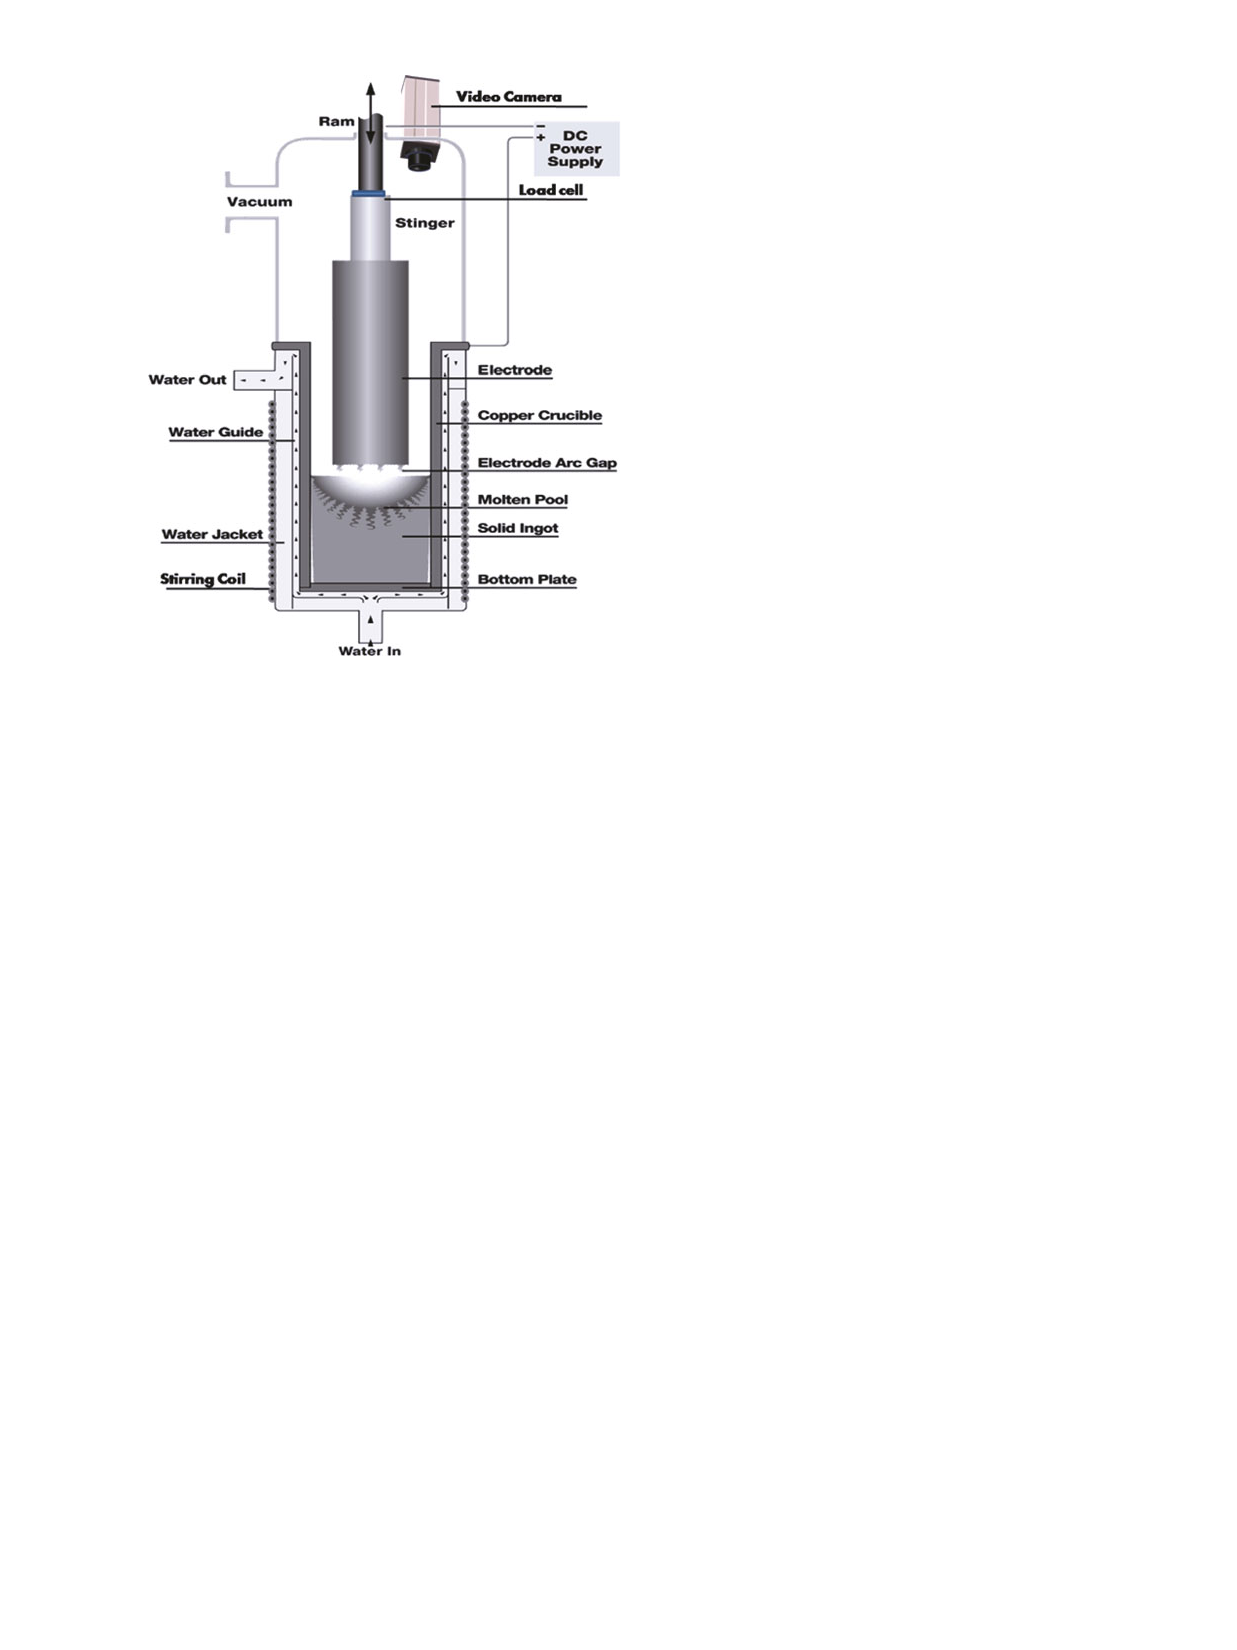
\includegraphics[width=0.45\textwidth]{furnace.pdf}
\caption{Cross section of VAR furnace. Image taken from Woodside et al.~\cite{Woodside:2013cf}}
\label{fig:vardiagram}
\end{figure}

% Challenge and Motivation
Arc behavior drives the remelting process and determines ingot quality, but arc positions are challenging to quantify due to the VAR system geometry and high-temperature environment.
Currently, video cameras directed down the annular gap between the electrode and crucible give operators qualitative information of arc behavior, as well as side arc detection, however these systems cannot track instantaneous arc formation and motion.
A robust arc detection and tracking system would give insight into the material properties of the final ingot.
A common approach for detailed study of VAR furnaces is numerical modeling~\cite{Gartling:1997ka,Reiter:2003wk,Wang:2005fg,Yang:2010kq,Zhao:2011es,Pericleous:2013kb,Woodside:2013cf,Beaman:2014fi}.
The application of large currents through the system results in a strong magnetic field surrounding the furnace, on which several studies focused~\cite{Wang:2005fg,Nair:2009ja,Woodside:2013cf}.
The arc position in the ingot-electrode gap is a key parameter that affects the magnetic field. 
Arcs concentrate the electrical current passing through the system and impact the distribution of the magnetic field.

% Lit Review
Mir et al.~\cite{Mir:2010cq} studied the thermal behavior of the consumable electrode using infrared cameras, focusing on heat transfer characteristics.
However, their technique required alteration of a furnace  and revealed little insight on arc behavior.
Zhao et al.~\cite{Zhao:2011es} used the two-dimensional FEM software ANSYS to study fluid dynamics in the molten pool.
The model assumed that only buoyant forces act on the melt pool, the melt pool exhibits turbulent flow properties, chemical reactions are negligible, and material properties depend only on temperature. 
They did not consider the effects of arc location on the melt pool, but mentioned it as a source of interest.
Gartling et al.~\cite{Gartling:1997ka} created a numerical model of the VAR process that delivered qualitatively accurate results. 
They emphasize one of the parameters that needed to be addressed are the characteristics of melt pool stirring due to electromagnetic, and therefore arc, characteristics. 
Reiter et al.~\cite{Reiter:2003wk} simulated heat transfer in VAR ingots during the melting process, where the coupling of an electromagnetic mathematical model was essential for accurate results. 
Pericleous et al.~\cite{Pericleous:2013kb} developed a three-dimensional transient multi-scale model that incorporated a macro-level FEM-based computational fluid dynamics model coupled with a microscale solidification model to study VAR processes.
They found that arc location and characteristics drive the occurrence of ``freckles'' and ``white spots,'' two key defects in the quality of VAR ingots~\cite{Pericleous:2013kb}.
Wang et al.~\cite{Wang:2005fg} developed a two-dimensional axisymmetric model to study arc characteristics under different axial magnetic fields using the commercially available software FLUENT. 
Their model focused on magnetohydrodynamics and plasma behavior in the electrode-ingot gap, assuming that plasma consisted of only electrons and ions and its flow can be described with a hydrodynamic approximation.  
They concluded that the effect of current density distribution, arc distribution, was significant for VAR because it directly correlates to the heat flux density at the anode.
Woodside et al.~\cite{Woodside:2010fi,Woodside:2013cf} used the multiphysics finite-element modeling (FEM) software COMSOL to simulate the magnetostatics of a VAR furnace.
They assumed an axisymmetric furnace, homogeneous material properties, and a single non-diffuse arc in a three-dimensional model.
Model results were used to develop a relationship between measured magnetic field readings at a notional Hall sensor position and arc locations~\cite{Woodside:2013cf}.
Nair et al.~\cite{Nair:2009ja} used the FEM software Opera3d to study the use of magnetic source tomography to understand arc behavior in VAR systems.
They modeled electrostatics while assuming homogeneous material properties, and included both single and double non-diffuse arcs.
Nair et al.\ concluded that arc locations can be predicted based on measurements of magnetic flux density outside the furnace with sufficient accuracy under the right circumstances. 
According to literature, arc locations and characteristics directly affect ingot characteristics.~\cite{Woodside:2013cf,Zhao:2011es,Nair:2009ja,Wang:2005fg,Pericleous:2013kb,Gartling:1997ka,Reiter:2003wk}
Various studies showed that arc locations can be predicted accurately using magnetic flux density measurements around VAR furnaces combined with accurate numerical models.~\cite{Woodside:2013cf,Nair:2009ja}
However, these methodologies made assumptions and simplifications that should be validated further to encourage their application in industry.

% Objectives of the study
The purpose of this study is to model the magnetostatics of the VAR process in different scenarios, while evaluating the impact of previously made assumptions, to determine the potential errors of arc locations predicted by the Arc Position Sensing (APS) system of Woodside and King~\cite{Woodside:2010fi}.
Understanding the behavior of the APS technology due to changing parameters could lead to further validation or improvement~\cite{Nair:2009ja,Woodside:2013cf}.
We used a multiphysics FEM simulation software to study the system. 
First, in Section~\ref{s:methods} we describe the methodology and approach used to establish a working model of the system, and discuss the methodology of the arc location prediction equations.
Next, in Section~\ref{s:results}, we inspect several factors that may impact the accuracy of arc location predictions, including the vertical distance between the sensor and arc, the size of the electrode-ingot gap, the effects of ingot shrinkage, and the use of multiple sensors.
Finally, in Section~\ref{s:conclusions} we summarize our results into primary conclusions, and make some recommendations of best practices for using---and further developing---the APS technology.

%%%%%%%%%%%%%%%%%%%%%%%%%%%%%%%%%%%%%%%%%%%%%%%%%%%%%%%%%%%%%%%%%%%%%%%%%%%%%%%%%%%%%%%%%%%%%%%%%%%%%%%%%%%%%%%%%%%%%%%%%%%%%%%%%%%

\section{Methodology}
\label{s:methods}

In this section, we describe our approach to modeling the VAR furnace and predicting arc locations based on model results.
We used the multiphysics FEM software COMSOL Multiphysics~\cite{COMSOL-4.3b} to simulate a simplified VAR furnace, with arcs located in different locations in the electrode-ingot gap.
Our model only considered magnetostatics, based on the steady-state Ampere's Law and current conservation equation:
\begin{align}
\mathbf{J} &= \nabla \times (\mu_0 ^{-1}\mu_r^{-1} \mathbf{B}) - \sigma \mathbf{v} \times \mathbf{B} \\
\mathbf{B} &= \nabla \times \mathbf{A} \\
\nabla \cdot \mathbf{J} &= 0 \;
\end{align}
where $\mathbf{J}$ is the current vector, $\mu_0$ is the permeability of a vacuum, $\mu_r$ is the relative permeability of the material, $\mathbf{B}$ is the magnetic flux density vector, $\sigma$ is the electrical conductivity, $\mathbf{v}$ is the particle velocity, and $\mathbf{A}$ is the magnetic vector potential.

\begin{table}[htbp]
\centering
\caption{Geometric specifications of modeled VAR furnace}
\begin{tabular}{@{}l l l@{}}
\toprule
	Component      & Radius (m)  & Height (m) \\
\midrule
	Electrode      & \num{0.381} & \num{1.000} \\
	Ingot          & \num{0.432} & \num{1.057} \\
	Crucible (outer) & \num{0.472} & \num{4.000} \\
	Crucible (inner) & \num{0.432} & \num{4.000} \\
	Furnace shell (outer) & \num{0.640} & \num{4.000} \\
	Furnace shell (inner) & \num{0.472} & \num{4.000} \\
	Arc            & \num{0.010} & \num{0.0254} \\
\bottomrule
\end{tabular}
\label{tab:geom}
\end{table}

\begin{figure}[htbp]
\centering
	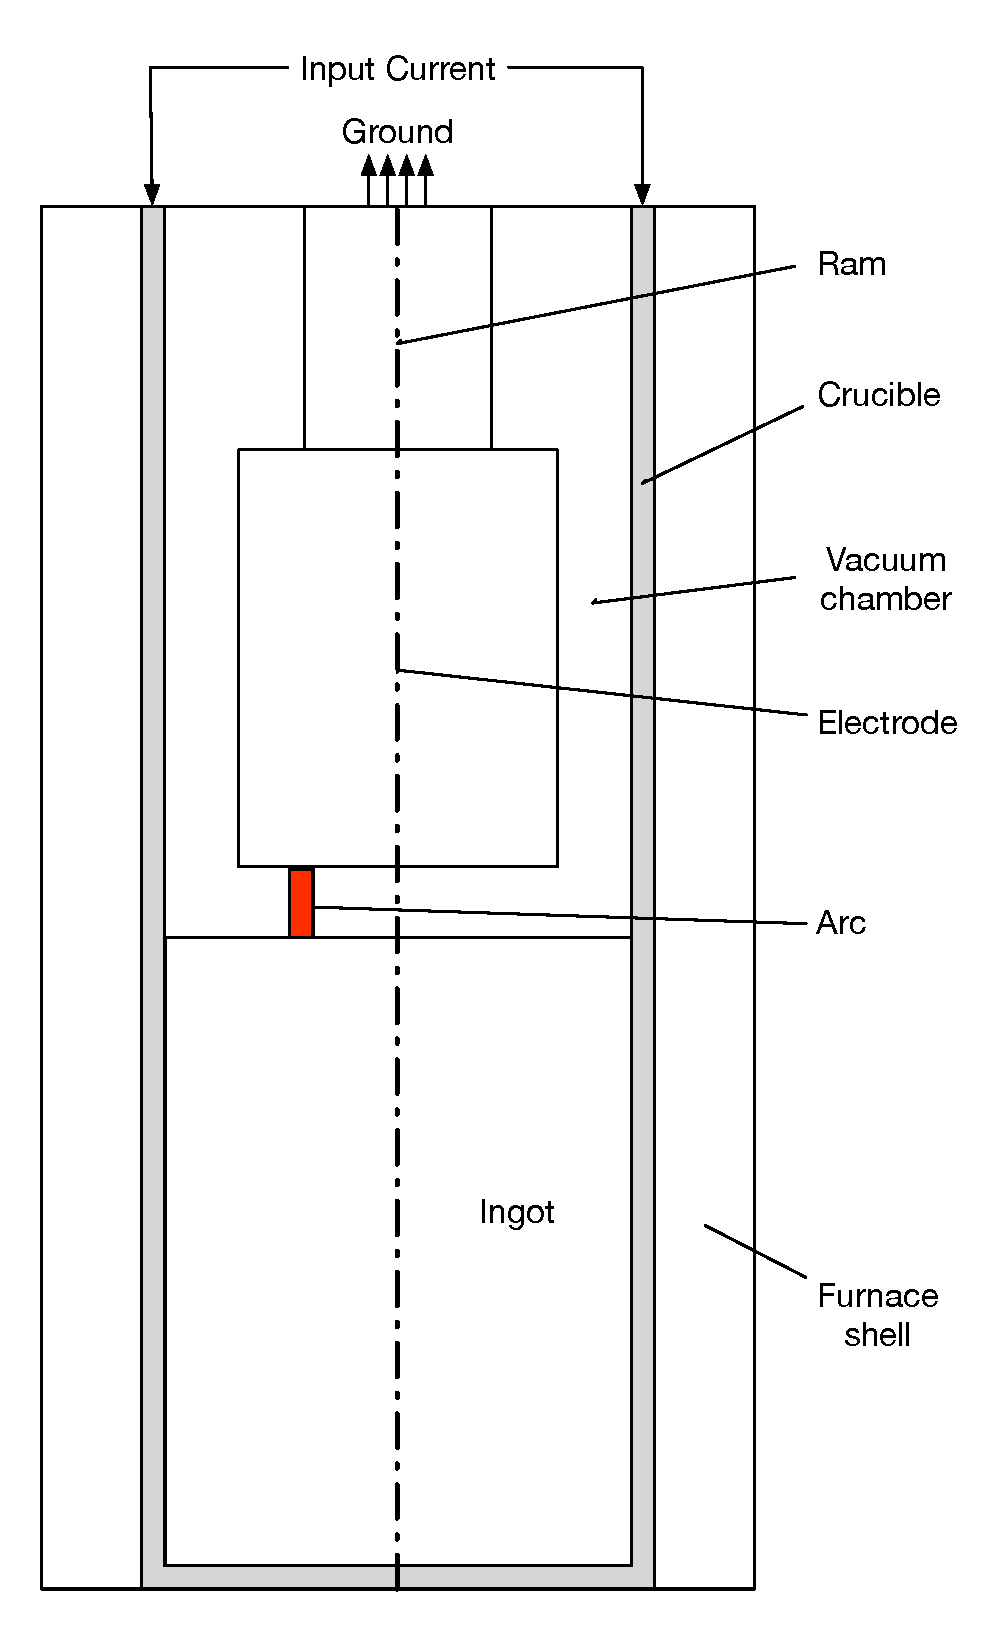
\includegraphics[width=0.5\textwidth]{VAR-diagram.pdf}
	\caption{Diagram of the geometry employed in the model (not to scale)}
	\label{fig:diagram}
\end{figure}

We modeled a simplified axisymmetric VAR furnace, based on the geometry of Woodside et al.~\cite{Woodside:2013cf}.
Table~\ref{tab:geom} lists the geometric specifications, and Fig.~\ref{fig:diagram} shows the geometry of the VAR furnace studied. 
%The geometric parameters for the furnace include: electrode radius of \SI{0.381}{\meter} and height of \SI{1.000}{\meter}, ingot radius of \SI{0.432}{\meter} and height of \SI{1.057}{\meter}, crucible thickness of \SI{0.04}{\meter} and height of \SI{4.000}{\meter}, external furnace shell radius of \SI{0.64}{\meter} (also radius of the sensor position) and height of \SI{4.000}{\meter}, constant arc radius of \SI{0.01}{\meter}, and ingot-electrode gap height of \SI{0.0254}{\meter}.
The electrode and ingot were both assumed to be titanium, with an electrical conductivity of \SI{7.407e5}{\siemens\per\meter} and relative permeability of \SI{7.9585e-7}{}.
The surrounding crucible was selected as copper (electrical conductivity of \SI{5.998e7}{\siemens\per\meter} and relative permeability of near \SI{1}{}), and the outer shell as steel (electrical conductivity of \SI{4.032e6}{\siemens\per\meter}, and relative permeability of near \SI{1}{}).
The annular space between the electrode and crucible and the electrode-ingot gap were modeled as near-vacuums, with an electrical conductivity of essentially zero (\SI{1e-15}{\siemens\per\meter}), and relative permeability of exactly \SI{1}{}. 
A small cylinder connecting the ingot and electrode represented the arc, with all current forced through that small location; the arc was assigned an electrical conductivity 20 orders of magnitude larger than its surroundings. 
The size of the cylinder has minimal effects on the magnetostatics of the scenario if its position and current remain constant.~\cite{Nair:2009ja}.
Another simplification applied to the model is the assumption that principles of superposition can be used in order to take into account the effects of multiple arcs.~\cite{Woodside:2013cf}.
The application of superposition was utilized by both Woodside et al. as well as Nair and Ward~\cite{Woodside:2013cf,Nair:2009ja}.
The top of the copper crucible was assigned a current source of \SI{35000}{\ampere}, and the system was grounded at the ram that feeds the electrode. 
Domain boundary conditions were set to mimic an infinite domain.
The entire domain used a mesh consisting of free tetrahedral cells, that was automatically determined by COMSOL.
We assigned the mesh size near the electrode-ingot gap as ``fine'' settings, with a minimum element size of \SI{0.0016}{\meter}.
The rest of the furnace geometry was set to ``medium'' settings, with a minimum element size of \SI{0.08}{\meter}.
The outer boundary was set to ``coarse'' mesh settings, with a minimum element size of \SI{0.224}{\meter}.
Mesh settings resulted in a total element count of approximately \num{170000}.
Further refining the grid changed solutions to within \SI{5}{\percent} of the results published here, so we selected the aforementioned settings as a tradeoff between acceptable accuracy and time-to-solution.

Next, we simulated sensor readings from one location.
We chose a point in the three-dimensional space of the domain to represent the sensor location; a physical sensor itself was not modeled, as its presence should not affect the magnetic field distribution.
We performed parametric sweeps of the arc location to calculate flux density changes at the sensor location. 
(Swept parameters in COMSOL include \emph{$r_0$} and $\theta_0$, where \emph{$r_0$} is the radial position of the arc from the center of the furnace and $\theta_0$ is the angular position of the arc with respect to the $x$-axis.) 
Figure~\ref{fig:large} shows the magnetic flux density ($T$) as a function of arc position for a sensor located at (\SI{0}{\meter},\SI{-0.64}{\meter}).

\begin{figure}[htbp]
\centering
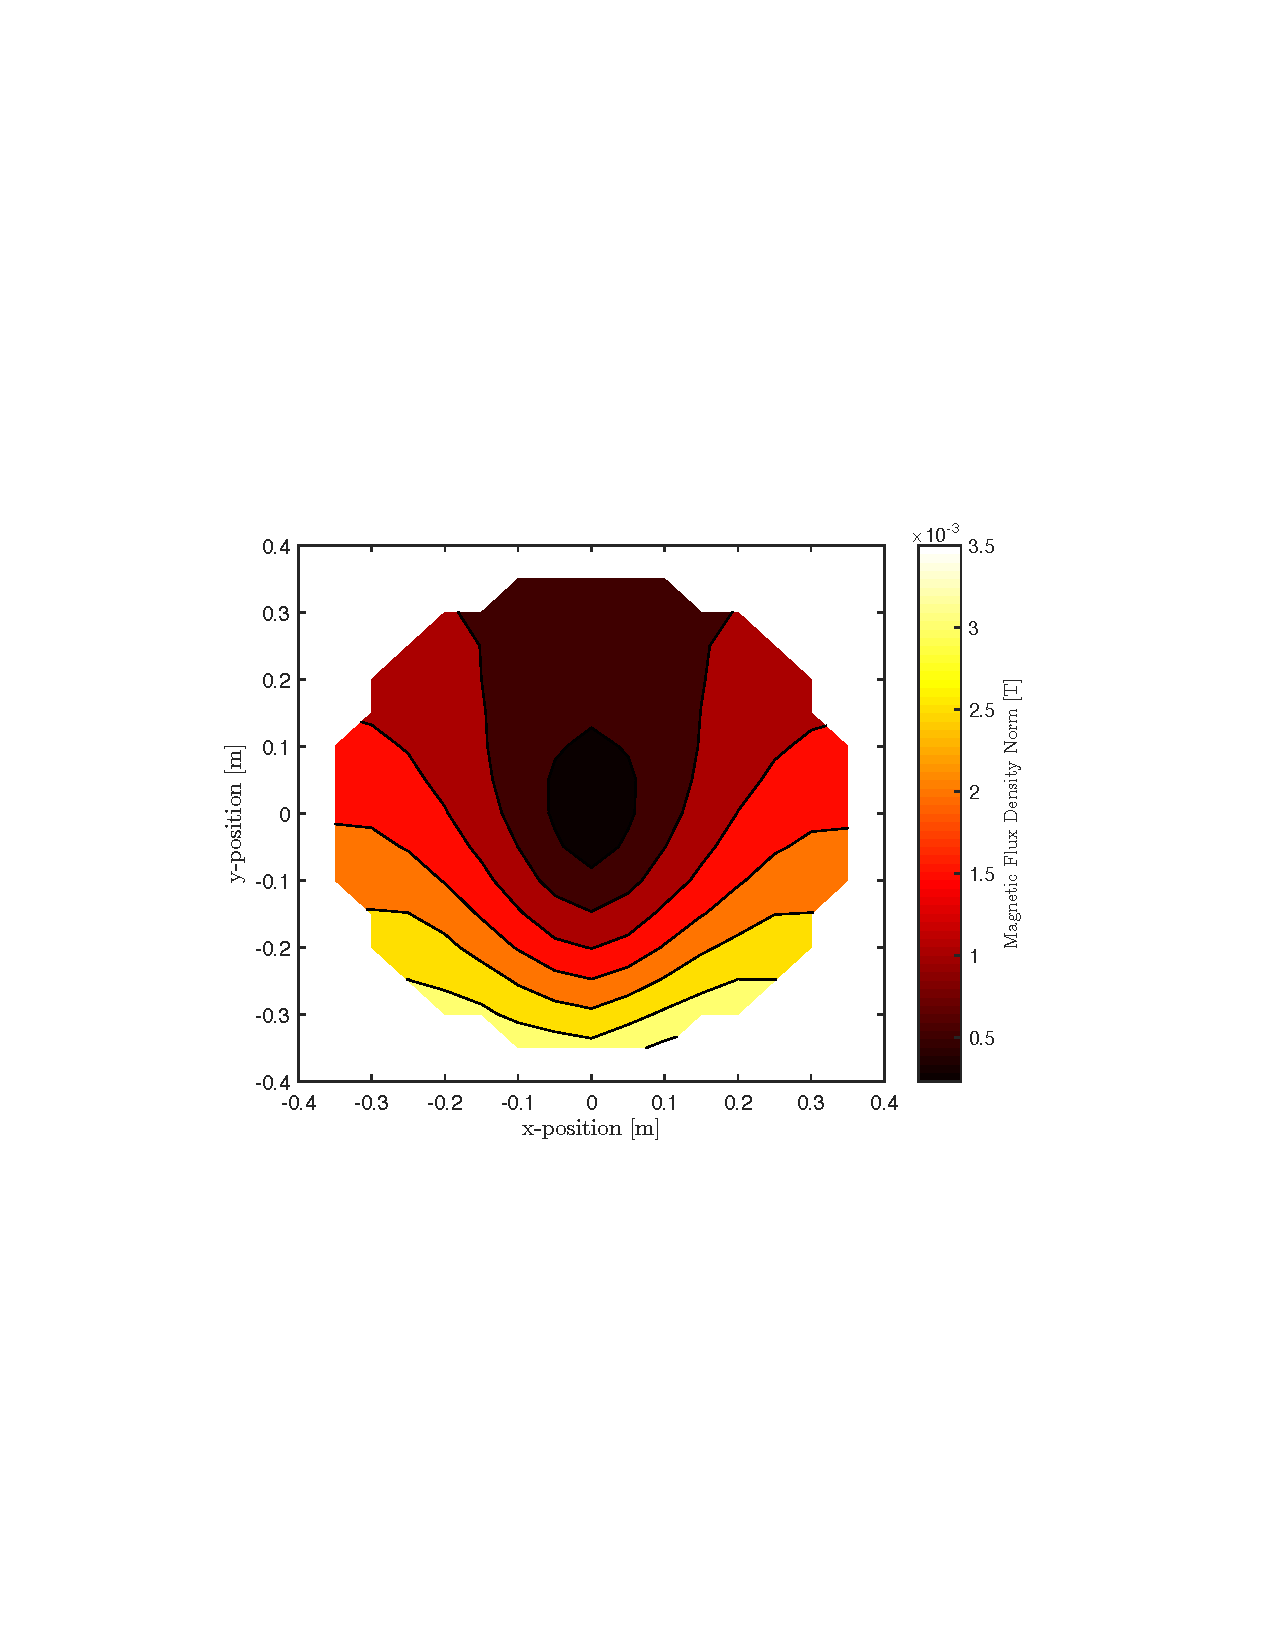
\includegraphics[width=0.6\textwidth]{Bnorm2.pdf}
\caption{Magnetic flux density norm with respect to arc location in Cartesian coordinates}
\label{fig:large}
\end{figure}

Arc position predictions can now be examined.
As determined by Woodside et al.~\cite{Woodside:2013cf} arc position determination can be achieved through the application of the Biot--Savart law. 
The Biot--Savart law with a magnetostatic derivation of the Maxwell--Ampere law, using the relation between superimposed line sources of current, and magnetic flux density vector $\mathbf{B}$ at a location $\mathbf{r}$ is given by
\begin{equation}
\mathbf{B}(\mathbf{r}) = \frac{\mu_0}{4 \pi} I \int \frac{d \mathbf{I}' \times \mathbf{\hat{r}}}{ \| \mathbf{r} \|^2 } \;,
\end{equation}
where $d \mathbf{I}'$ is an element of the length along the total current, $\mathbf{r}$ is the vector from the source to the point, and $\mathbf{\hat{r}}$ is the unit vector of $\mathbf{r}$.
This equation can be used to find the components of the magnetic field:
\begin{align}
\mathbf{B}_t &= m_t I \left( \sum \frac{f_i \sin \theta_i}{d_i} - \frac{1}{r_s} \right) \;, \text{ and} \label{eq:magnetic_t} \\
\mathbf{B}_r &= m_r I \left( \sum \frac{-f_i \cos \theta_i}{d_i} \right) \;. \label{eq:magnetic_r}
\end{align}
where $\mathbf{B}_t$ and $\mathbf{B}_r$ are the tangential and radial components of the magnetic flux density, $m_t$ is the tangential furnace coefficient, $m_r$ is the radial furnace coefficient, $I$ is the line current, $\theta_0$ is the input angle in the model of an arc, from the center of the furnace, $d_0$ is the input radius of an arc, from the center of the furnace, $\theta_i$ is the angle from the sensor to the arc location, $d_i$ is the length from the sensor to the arc location, $r_s$ is the distance from the sensor to the center of the furnace, and $f_i$ is the fraction of the total current associated with the arc.

\begin{figure}[htbp]
\centering
	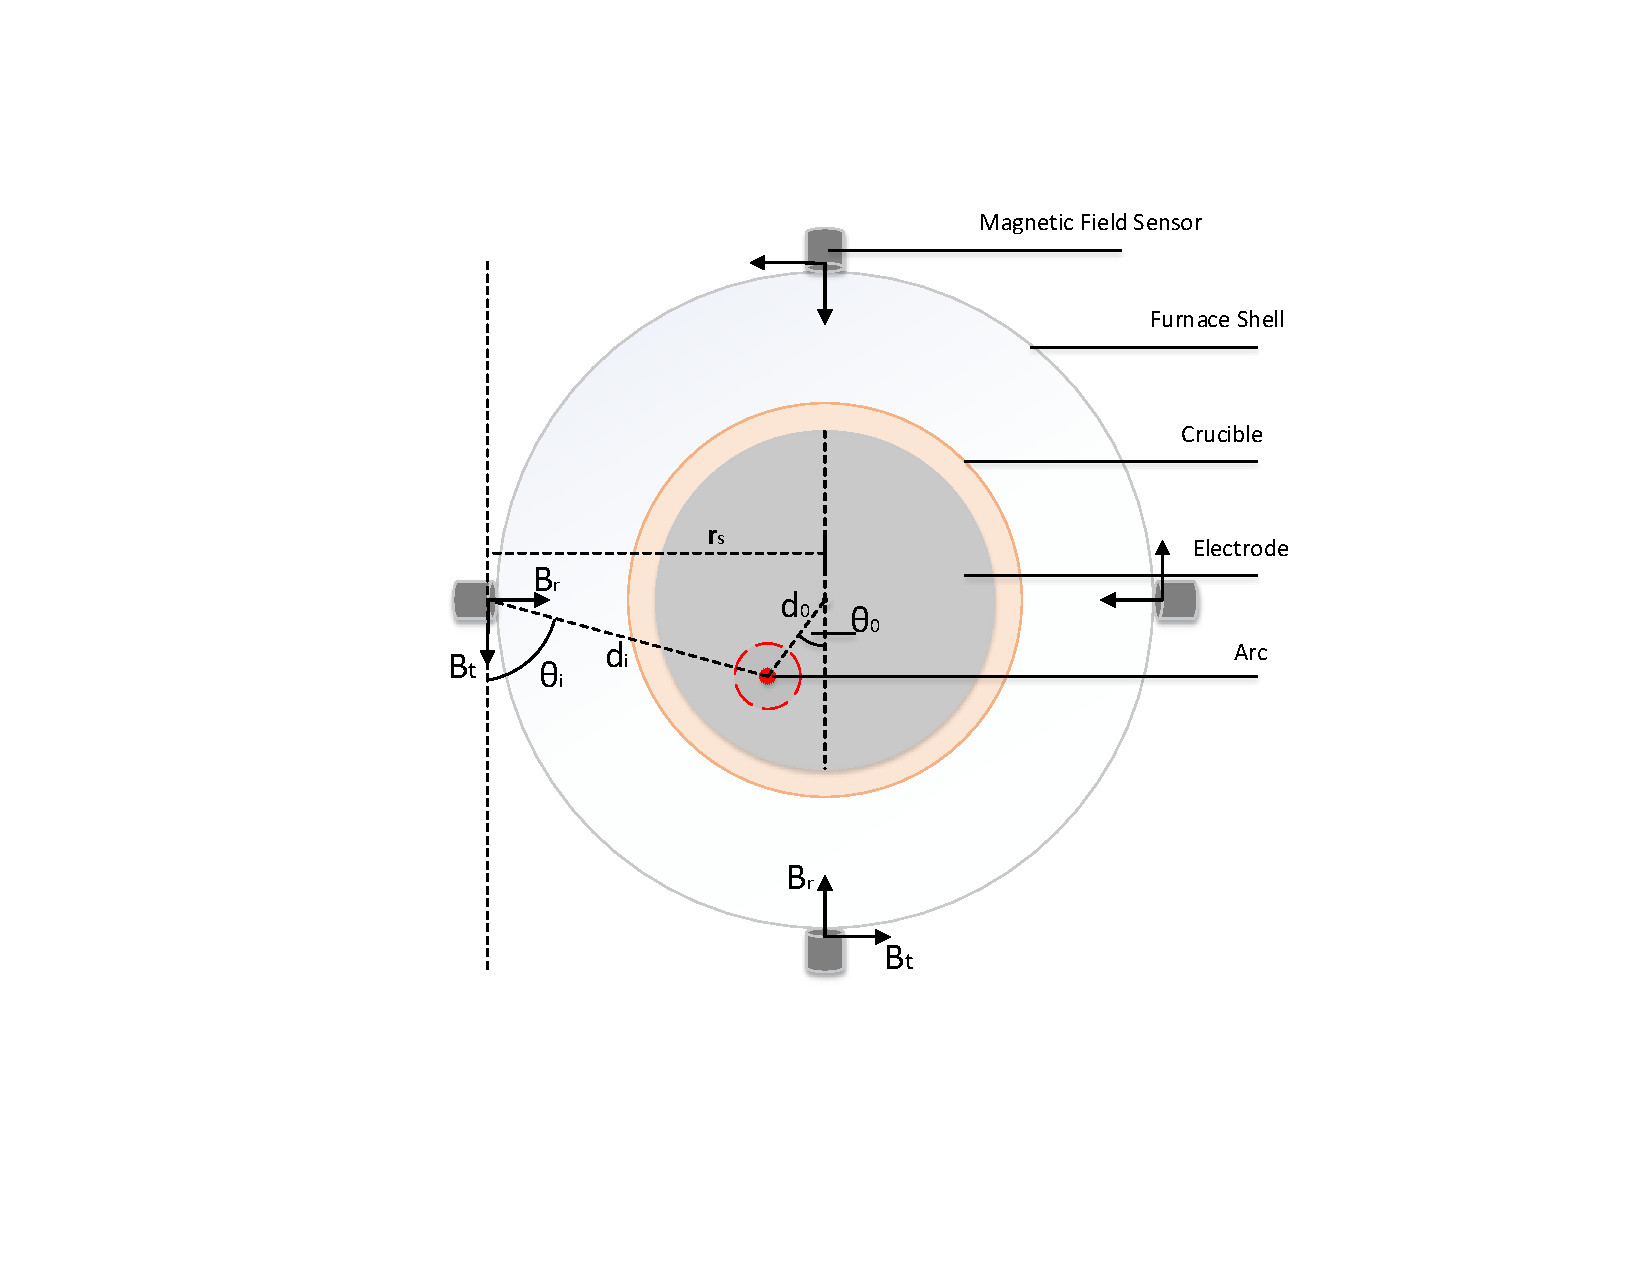
\includegraphics[width=0.6\textwidth]{diagram1.pdf}
	\caption{Overhead cross-sectional diagram of a VAR furnace, shown with four two-axis magnetic field sensors and the geometry of the variables for one sensor}
	\label{fig:cross_section}
\end{figure}

Figure~\ref{fig:cross_section} shows a top-down cross-section of the VAR furnace modeled, including sensor locations.
The furnace coefficients $m_t$ and $m_r$ depend on the geometry and configuration of individual furnaces~\cite{Woodside:2013cf}.
The input angle for the COMSOL model and the angle $\theta$ are different measurements. 
Using the Biot--Savart equations, a nonlinear regression was used to determine the unknown furnace coefficients $m_t$ and $m_r$.
Once these were determined, the single-line current versions of the Biot--Savart equations were solved for $d_i$ and $\theta_i$ (according to Fig.~\ref{fig:cross_section}) with input or measured magnetic flux density components.
A vector reference frame rotation and translation is done to transform the magnetic field values from the reference of the center of the furnace to each sensor location.
The equations take the form
\begin{align}
d_i &= \frac{I m_r m_t}{\sqrt{{\frac{I^2 m^2_r m^2_t}{r^2_s}}+\frac{2 I B_t m_t m^2_r}{r_s} + B^2_r m^2_t + B^2_t m^2_r}} \;, \text{ and} \label{eq:arc_diameter} \\
\theta_i &= \cos^{-1} \left( \frac{-B_r d_i}{m_r I} \right) \;. \label{eq:arc_angle}
\end{align}

\begin{figure}[htbp]
	\centering
	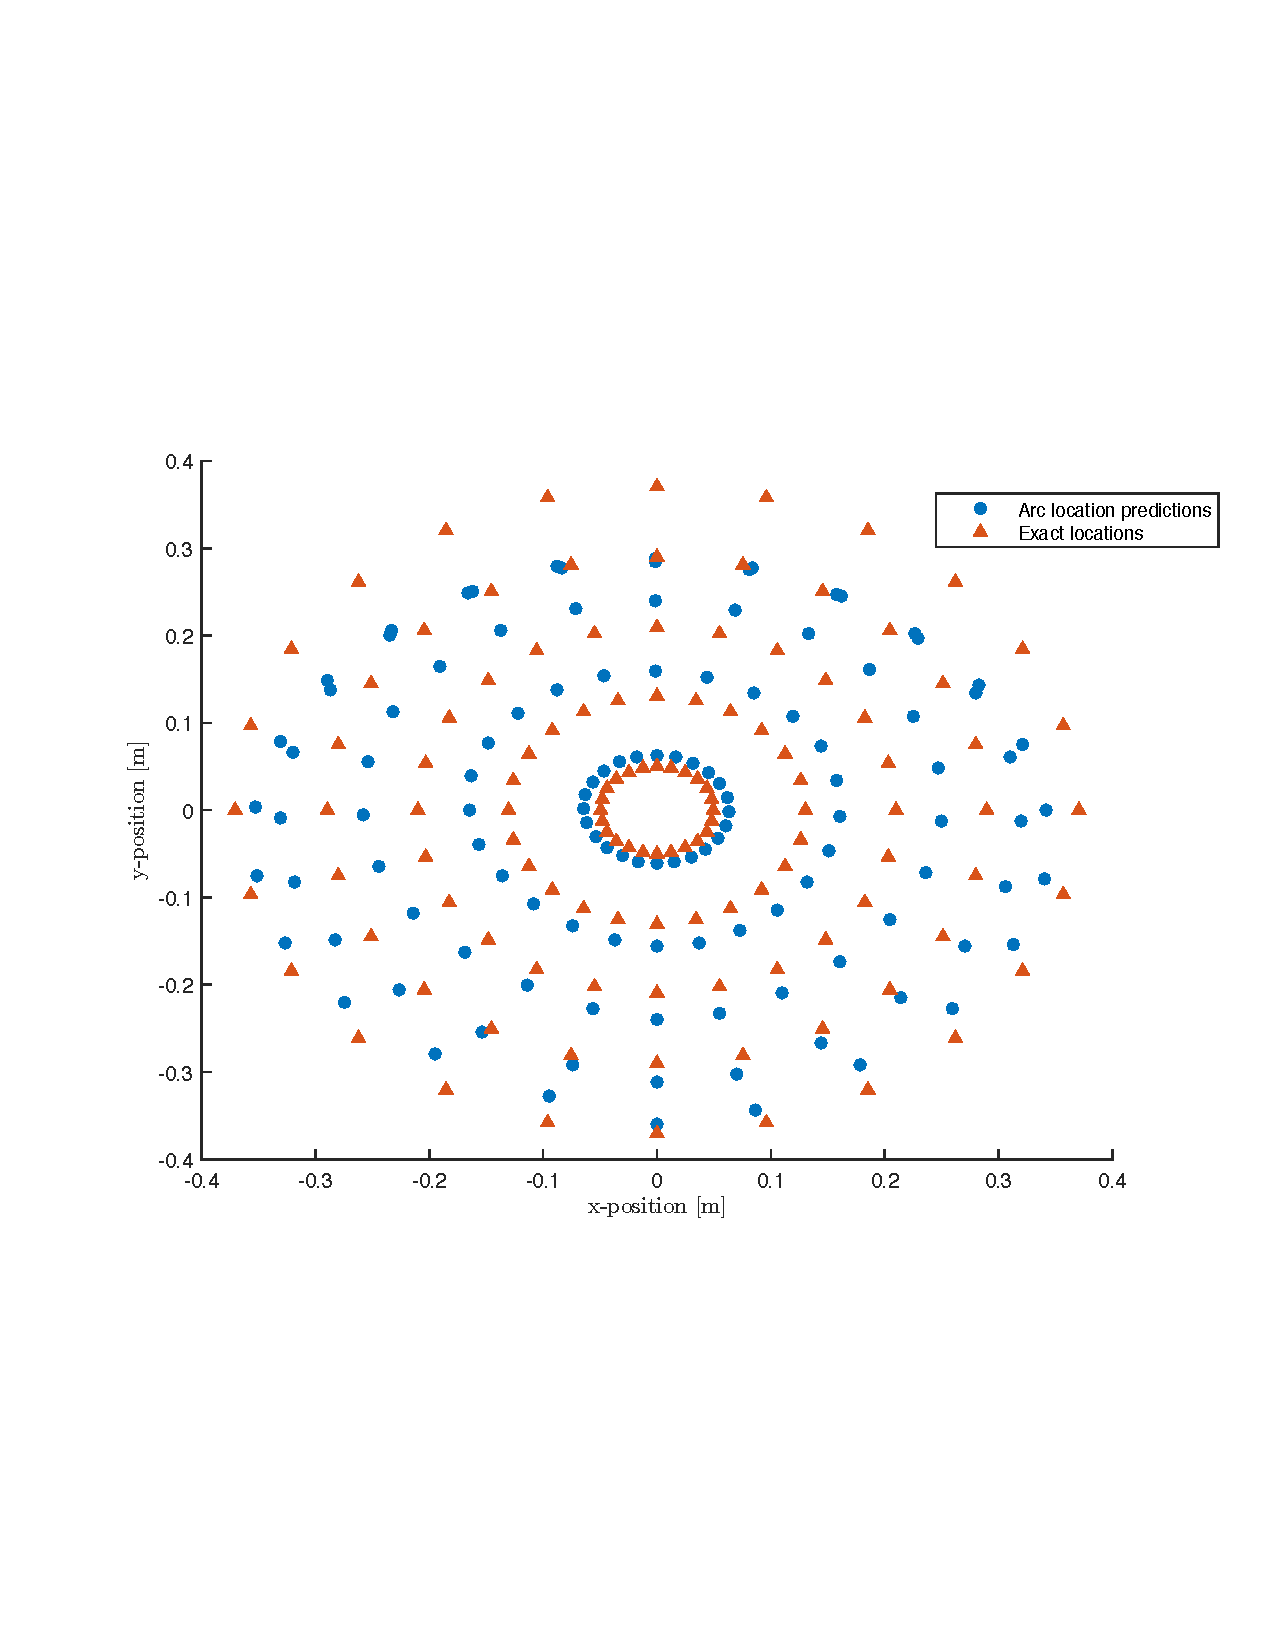
\includegraphics[width=0.7\textwidth]{OneSensorExpected2.pdf}
	\caption{Predicted arc locations compared to exact locations (calculated using furnace coefficients $m_r$ = \SI{8.15e-8}{\newton\per\ampere\squared}, $m_t$ = \SI{4.98e-8}{\newton\per\ampere\squared})}
	\label{fig:exactpos}
\end{figure}

These equations represent the basis of the APS technology~\cite{Woodside:2013cf}; using a given geometry and FEM-based furnace coefficients, the arc can be located using measurements of magnetic flux density and the current through the system. 
Performing a parametric sweep of arc locations in the model results in magnetic flux density components at the sensor location.
This array of values is equivalent to experimentally measured sensor magnetic flux density values.
Figure~\ref{fig:exactpos} shows the predicted arc locations in contrast to the exact locations. 
Table~\ref{tab:new_coeffs} compares the furnace coefficients found here with those of Woodside et al.~\cite{Woodside:2013cf}; our implementation predicts arc locations within five percent of the published values. 
This discrepancy likely resulted from slight differences in geometry or solver setup (we developed our model based on published descriptions), differing COMSOL versions, or a different selection of input arc locations to calculate the furnace coefficients.

\begin{table}[htbp]
\centering
\caption{Comparison of furnace coefficients from Woodside et al.~\cite{Woodside:2013cf} with those determined here}
\begin{tabular}{@{}l l l@{}}
\toprule
	& \emph{$m_r$} (\si{\newton\per\ampere\squared}) & \emph{$m_t$} (\si{\newton\per\ampere\squared}) \\
\midrule
	FEM results & $8.15\times10^{-8}$ & $4.98\times10^{-8}$ \\
	Woodside et al.\ & $9\times10^{-8}$ & $4.9\times10^{-8}$ \\
\bottomrule
\end{tabular}
\label{tab:new_coeffs}
\end{table}

The remaining sections of the paper describe the performance of the arc position sensing approach as various model parameters are varied or assumptions are relaxed.
This performance is described in terms of percent error in the predicted arc locations with respect to the known arc locations, normalized by the ingot radius (\SI{0.432}{\meter}).
The error is determined as the difference between two position vectors, the predicted and exact locations of the arc. 
\begin{align}
	error = \frac{\sqrt{(x - \hat{x})^2 + (y - \hat{y})^2}}{radius_{ingot}}*100
\end{align}

where $x$, $y$ are the exact positions and $\hat{x}$, $\hat{y}$ are the predicted positions.

%%%%%%%%%%%%%%%%%%%%%%%%%%%%%%%%%%%%%%%%%%%%%%%%%%%%%%%%%%%%%%%%%%%%%%%%%%%%%%%%%%%%%%%%%%%%%%%%%%%%%%%%%%%%%%%%%%%%%%%%%%%%%%%%%%%

\section{Results and discussion}
\label{s:results}

In this section, we describe the results of our studies on the impact of various factors on the accuracy of arc location predictions.
We considered the effects on arc location predictions of vertical sensor position (i.e., relative vertical distance between the sensor and arc), electrode-ingot gap size, ingot shrinkage, and using the average of predictions from multiple sensors.
All error calculations were based on the difference between the known position specified in the COMSOL model and the location predicted using Eqs.~\eqref{eq:arc_diameter} and \eqref{eq:arc_angle}.

%%%%%%%%%%%%%%%%%%%%%%%%%%%%%%%%%%%%%%%%%%%%%%%%%%%%%%
\subsection{Effect of vertical sensor position}
\label{sec:vertical_position}
%%%%%%%%%%%%%%%%%%%%%%%%%%%%%%%%%%%%%%%%%%%%%%%%%%%%%%

%First, we considered the impact of the sensor being position 
The original APS studies of Woodside et al.~\cite{Woodside:2010fi,Woodside:2013cf} considered a single sensor located in the plane of the electrode-ingot gap, where theoretically the most accurate results would be achieved due to the line-current source assumption.
In reality, due to the continuous movement of the electrode and growth of the ingot, the sensor would be in that plane only for a small amount of time relative to the the entire process.
In addition, Ingots used for industrial VAR applications can be several meters in length amplifying any error caused by deviation from the electrode-ingot gap. 
A solution to this problem is the application of multiple rings of sensor installed in intervals that lie within acceptable error.
We therefore want to quantify the potential error induced by a vertical separation between sensor and arc, in order to decide how frequently or far apart sensors should be placed along a furnace.
To determine the error of vertical distance between the arc and sensor, we varied the vertical sensor position away from the plane of the gap in multiples of the electrode-ingot gap height: $\pm$\numlist{0;1;2;3;5;7;10;15;20}.

\begin{figure}[htbp]
	\centering
	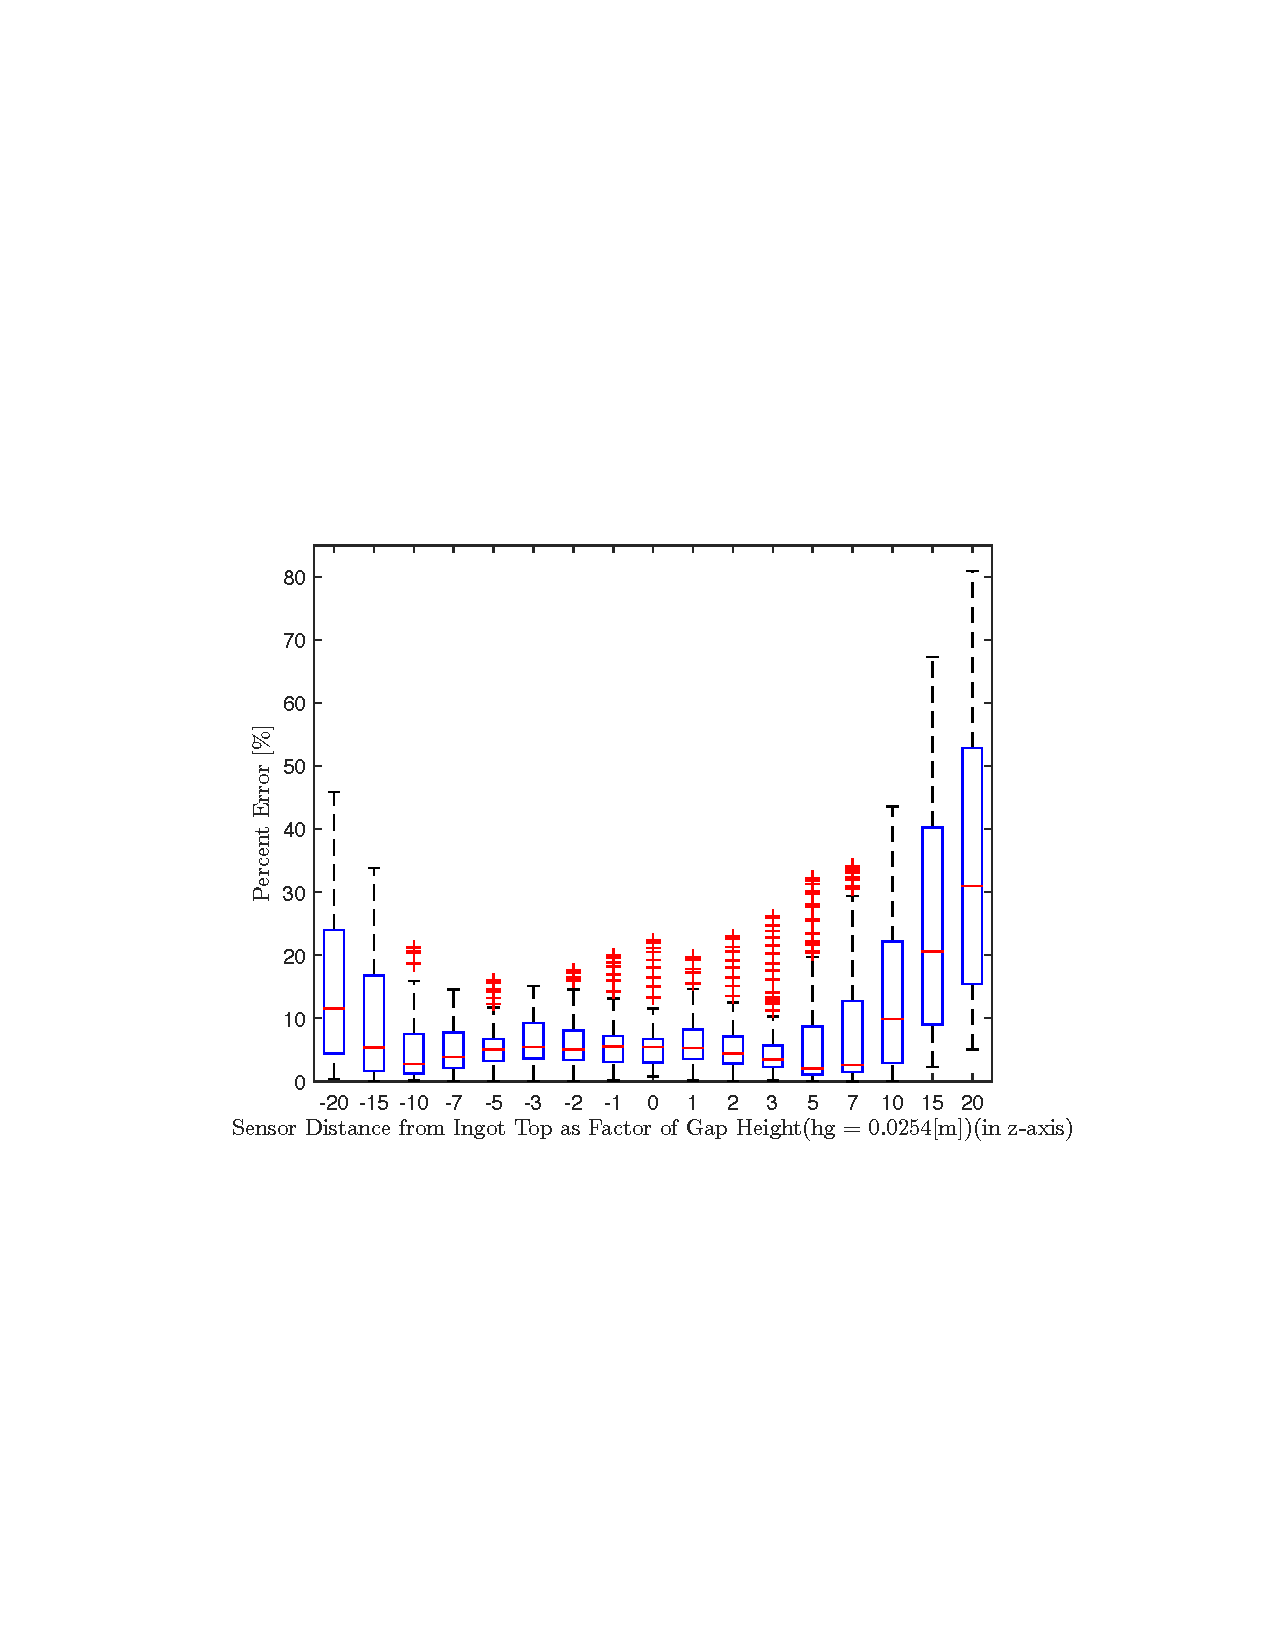
\includegraphics[width=0.6\textwidth]{constant_furnace_coef_sensorheight_error.pdf}
	\caption{Statistical error distribution of predicted arc locations with respect to vertical sensor position using constant furnace coefficients}
	\label{fig:avg_error}
\end{figure}

Figure~\ref{fig:avg_error} shows a box-and-whisker statistical distribution of the percent error in predicted arc position with respect to vertical sensor position using a single sensor; clearly, the error increases both as the sensor moves above and below the gap.
The red line inside the rectangles represents the median, the blue boxes span the 25th and 75th percentiles of the data, and the black whiskers span the maximum and minimum values not defined as outliers.
Outliers---defined as values greater than three times the standard deviation---are represented by red plus-sign markers.
Interestingly, the trend in increasing error is asymmetric, with error increasing more rapidly for sensor locations above the gap.
The asymmetry observed in error is most likely caused by the asymmetry of the current loop in the system. 
The reasons for the error being lower for sensors below the electrode-ingot gap is not clear. 


\begin{figure}[htbp]
	\centering
	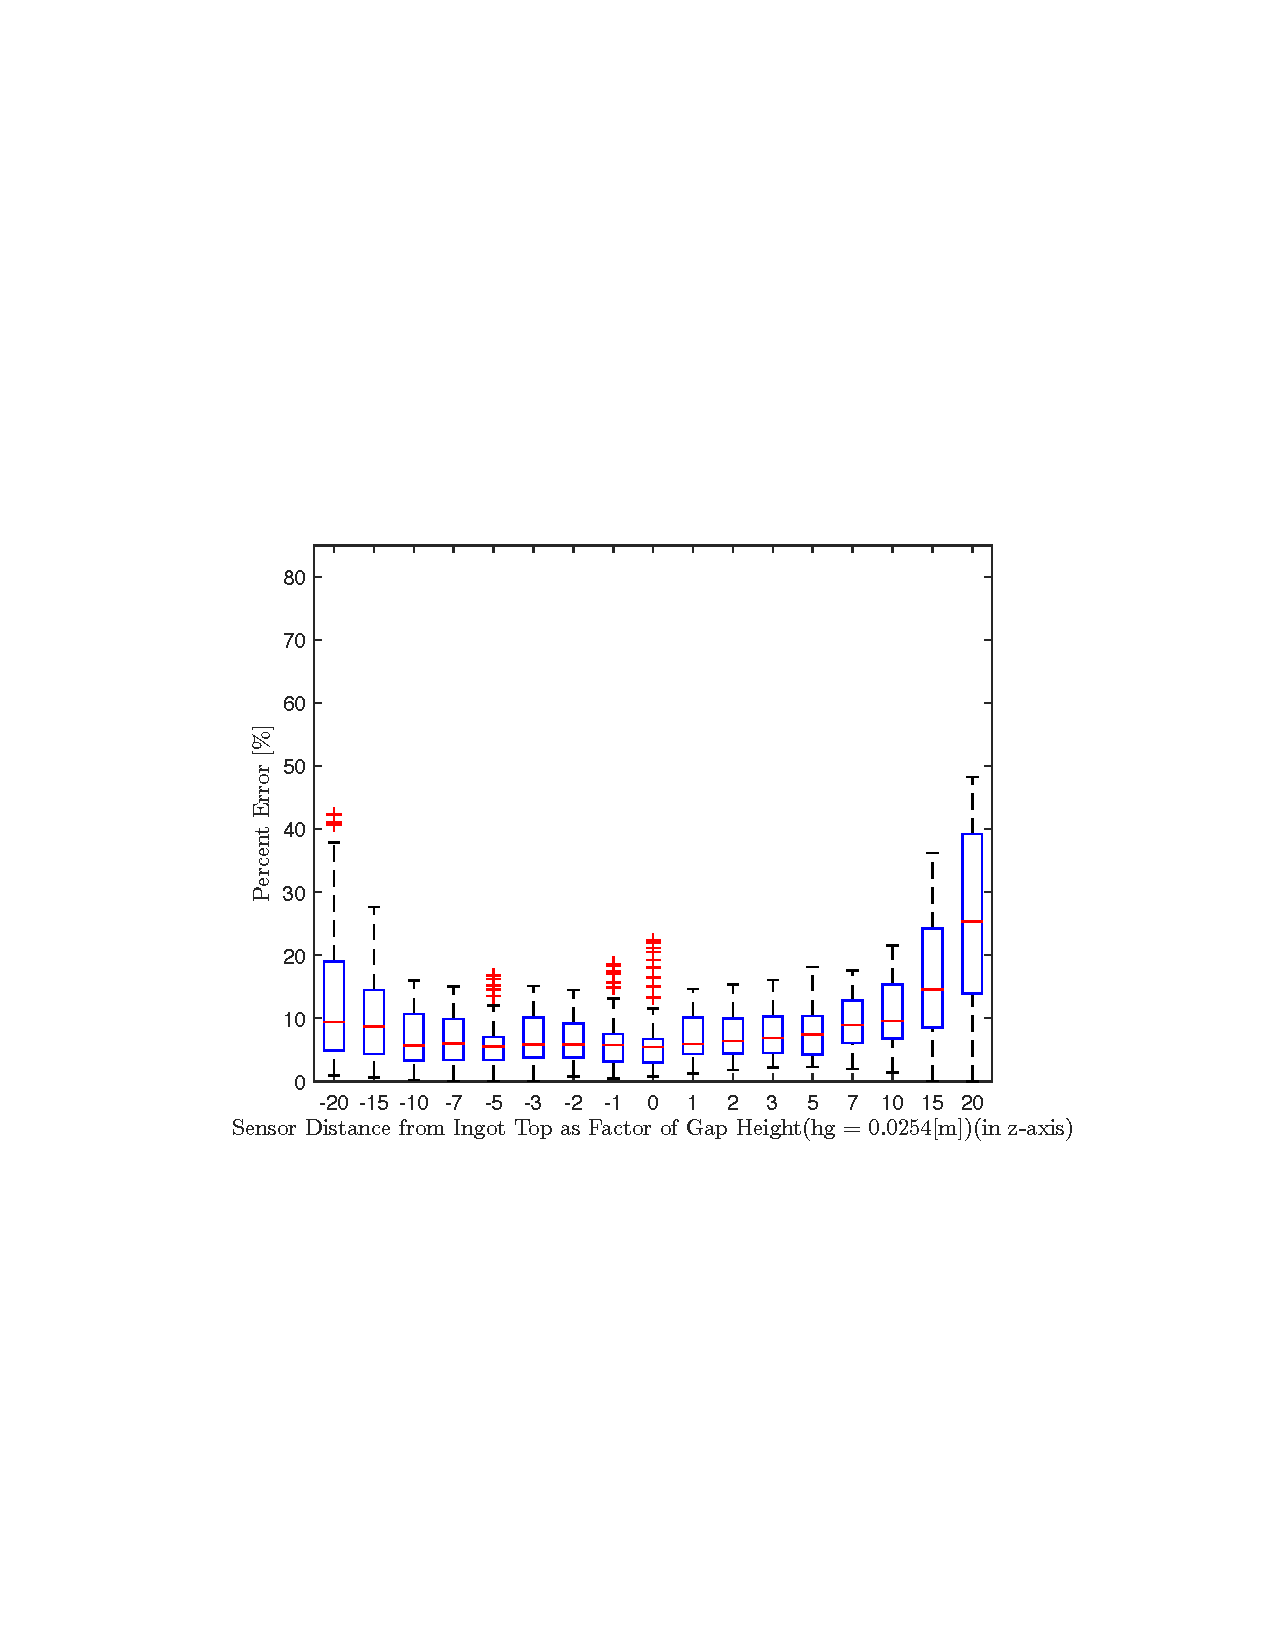
\includegraphics[width=0.6\textwidth]{variable_furnace_coef_sensorheight_error.pdf}
	\caption{Error distribution of predicted arc locations with respect to vertical sensor position using adaptive furnace coefficients}
	\label{fig:vavg_error}
\end{figure}

For the results shown in Fig.~\ref{fig:avg_error}, arc locations were predicted assuming constant furnace coefficients determined using data for a sensor placed at the plane of the electrode-ingot gap.
We can also recalculate coefficients for each sensor location, and investigate whether this practice improves results. 
This procedure is identical to that of the normal coefficient calculation, but uses magnetic flux density measurements at the various vertical sensor locations (rather than in the plane of the gap).
Figure~\ref{fig:vavg_error} shows the distribution of error in predicted arc locations using furnace coefficients recalculated for each sensor location.
The varying furnace coefficients aided in suppressing outliers, and reducing maximum error.
For the sensor position of $20 \times$ $h_g$, using varying coefficients reduced maximum error by more than \SI{30}{\percent}, and decreased median error by approximately \SI{5}{\percent}.
Median error shows a slight increase for all vertical sensor positions; however, using varying furnace coefficients reduced the overall distribution of error. 
The application of varying furnace coefficients decreased maximum error by \SI{9.27}{\percent} on average for all sensor locations, compared to using constant coefficients.
Looking at four points in more detail, for a sensor located $5 \times$ above and below the gap, median error for variable coefficients increased by \SI{5.43}{\percent} and decreased by \SI{0.46}{\percent} respectively, compared to their constant coefficient counterparts. 
For a sensor located $10 \times$ above and below the gap, median error decreased by \SI{0.31}{\percent} and increased by \SI{2.92}{\percent}, respectively. 
In real world systems the true vertical position of the electrode-ingot gap is unknown, however reasonable estimates can be made using data from the melt such as weight and size of the ingot, time, and ram position. 
Including this step in the algorithm could result in higher accuracy as shown in the results, however it would require real-world testing and experimentation to confirm. 

%for a sensor located $5 \times$ above the gap, median error increased by \SI{5.43}{\percent}; for a sensor located $5 \times$ below the gap, median error decreased by \SI{0.46}{\percent}. 
%When the sensor is located $10 \times$ above the gap, median error decreased by \SI{0.31}{\percent}, and for a sensor %located $10 \times$ below the gap median error increased by \SI{2.92}{\percent}.

% I don't think this plot is that useful.

%Error distributions give some indication of the behavior of predictions with sensor position height, but more information may be obtained by studying the error of individual arc positions.
%Figure~\ref{fig:inder} shows the error in predictions of five specific arc locations (out of the total 120).
%For sensor positions within \SI{\pm 0.2}{\meter} from the plane of the electrode-ingot gap, the errors in predicted arc locations vary within approximately \SIrange{0}{3}{\percent}, but with no discernible pattern.
%However, for sensors positioned further above or below the gap plane, the errors in predicted location increase monotonically with increasing arc distance from the furnace center.
%For a sensor located \SI{9999}{\meter} above the gap, arc location is predicted $8.3 \times$ worse for an arc located $2.8 \times$ further from the center (comparing the arcs located at \SI{0.13}{\meter} and \SI{0.37}{\meter} from the center).
%\todo[inline]{this sentence still needs some data}

%\begin{figure}[htbp]
%	\centering
%	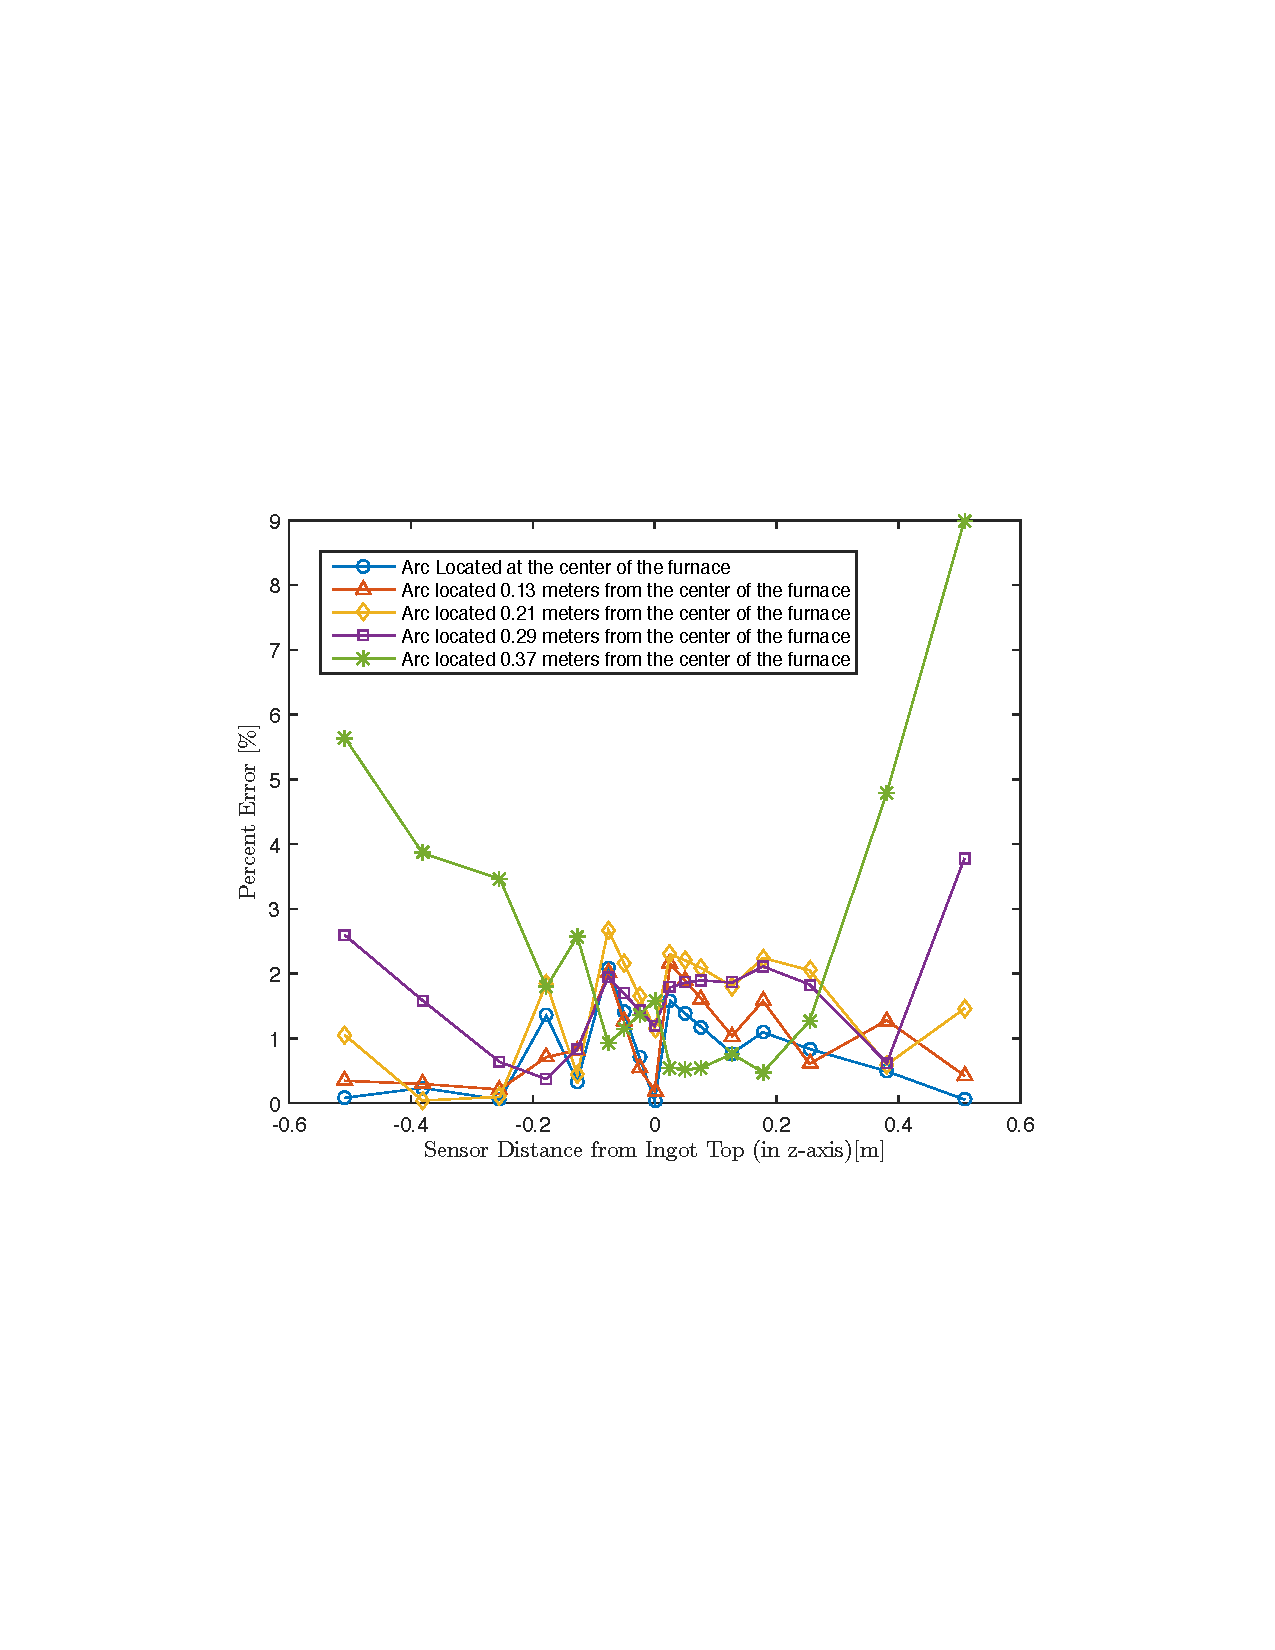
\includegraphics[width=0.6\textwidth]{indiv_arcerror.pdf}
%	\caption{Percent error of individual arc locations, while varying the arc position from the center of the furnace towards the sensor location}
%	\label{fig:inder}
%\end{figure}

While percent error at each location offers some information about measurement accuracy, examining the actual predicted locations and how they change can give insight on trends. 
Figure~\ref{fig:trends} shows arc location predictions as the sensor location moves from the electrode-ingot gap plane upwards along the furnace wall, for vertical sensor locations of \SIlist{0;0.0762;0.254;0.508}{\meter} (or \numlist{0;3;10;20} $h_g$).
As the sensor position moves away from the electrode-ingot gap, the arc location predictions cluster together near the center of the furnace. 
We hypothesize that this results from the current density concentrating inwards inside the electrode as it traverses through the electrode and into the smaller-radius ram.
The equations used to locate arc positions are two dimensional, using tangential and radial magnetic flux values in the plane of the sensor's vertical position.
The magnetic flux values measured by sensors positioned away from the electrode-ingot gap plane are small; for example, a sensor positioned at the electrode-ingot gap plane, a maximum of \SI{3.3e-3}{\tesla} in the radial direction and \SI{3.5e-3}{\tesla} in the tangential direction are observed.
On the other hand, a sensor located \SI{0.5}{\meter} above the electrode-ingot gap measures a maximum of \SI{2.5e-4}{\tesla} in the radial direction and \SI{7.5e-4}{\tesla} in the tangential direction.
In Eqs.~\ref{eq:arc_diameter} and~\ref{eq:arc_angle} used to calculate position, magnetic flux components appear in the denominator---so the order-of-magnitude smaller values at the higher sensor location result in predicted locations further away.
However, Fig.~\ref{fig:trends} shows that the location predictions shift further away and also cluster around the center of the furnace.
This supports the hypothesis that the electrical current funnels as it traverses the electrode, and the magnetic flux density values being measured at sensor locations away from the gap is the current density in the electrode for that plane.
This clustering behavior would impact results by indicating the presence of arcs near the center of the furnace, when they might actually occur near the edges of the electrode and ingot.


\begin{figure}[htbp]
	\centering
	\begin{subfigure}[b]{0.495\textwidth}
	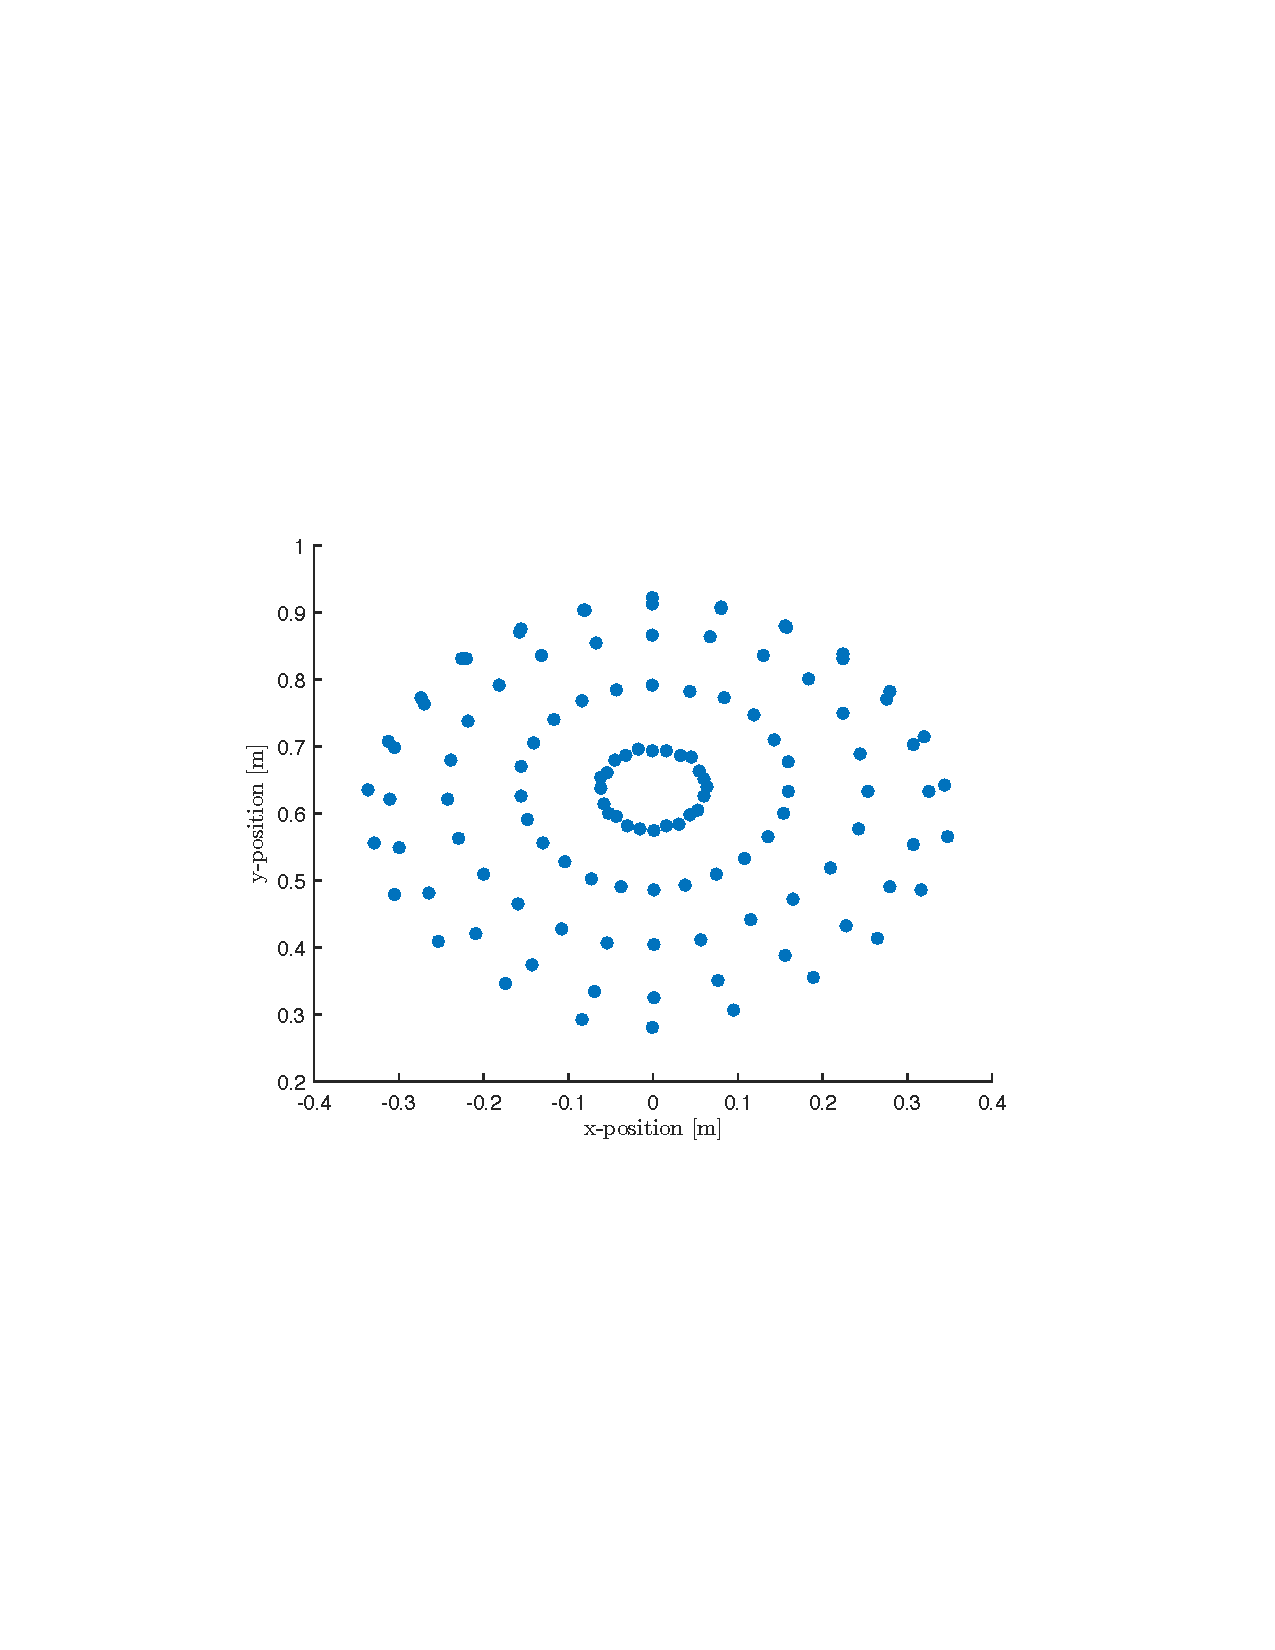
\includegraphics[width=\textwidth]{sh1.pdf}
	\caption{Arc location prediction with a sensor at the electrode-ingot gap (\SI{0}{\meter} above the electrode-ingot gap)}
	\end{subfigure}
	\hfill
	\begin{subfigure}[b]{0.495\textwidth}
	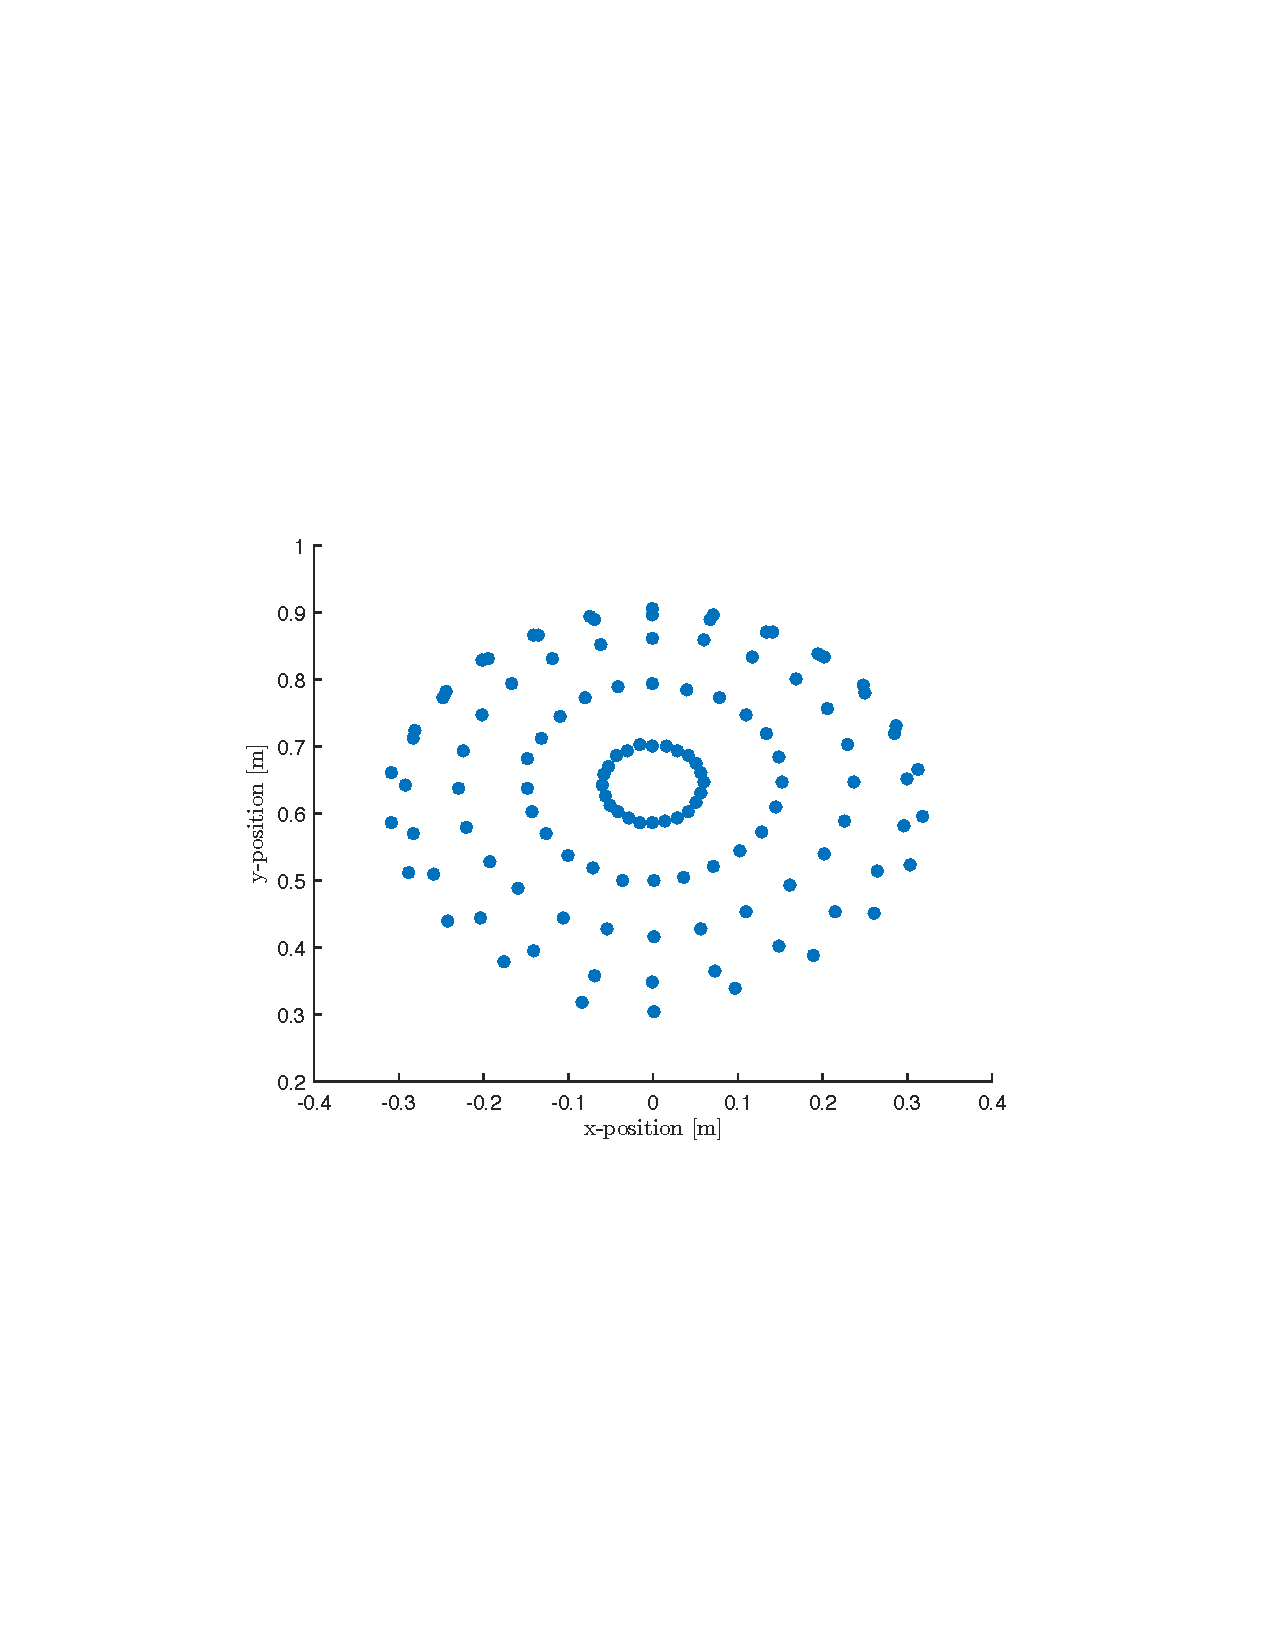
\includegraphics[width=\textwidth]{sh2.pdf}
	\caption{Arc location prediction with a sensor \SI{0.0762}{\meter} above the electrode-ingot gap}
	\end{subfigure}
	\\
	\begin{subfigure}[b]{0.495\textwidth}
	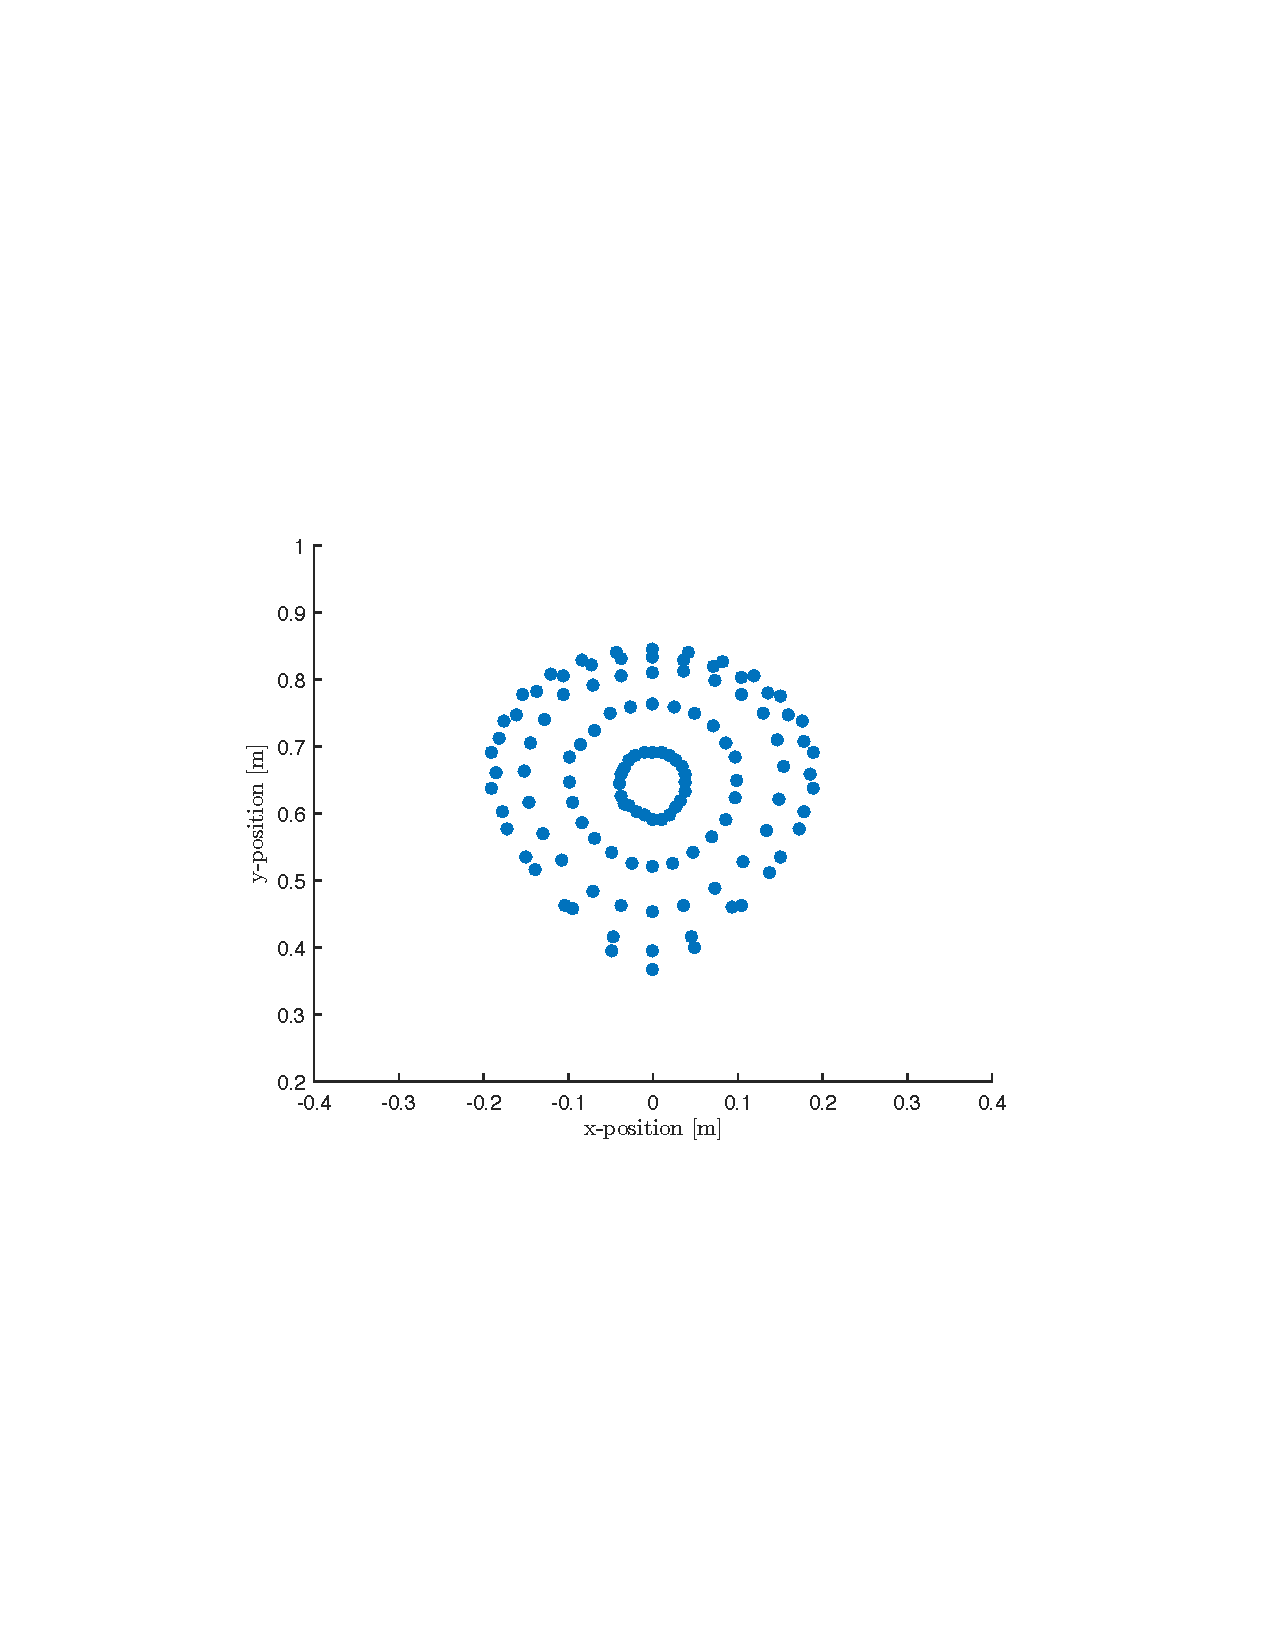
\includegraphics[width=\textwidth]{sh3.pdf}
	\caption{Arc location prediction with a sensor \SI{0.254}{\meter} above the electrode-ingot gap}
	\end{subfigure}
	\hfill
	\begin{subfigure}[b]{0.495\textwidth}
	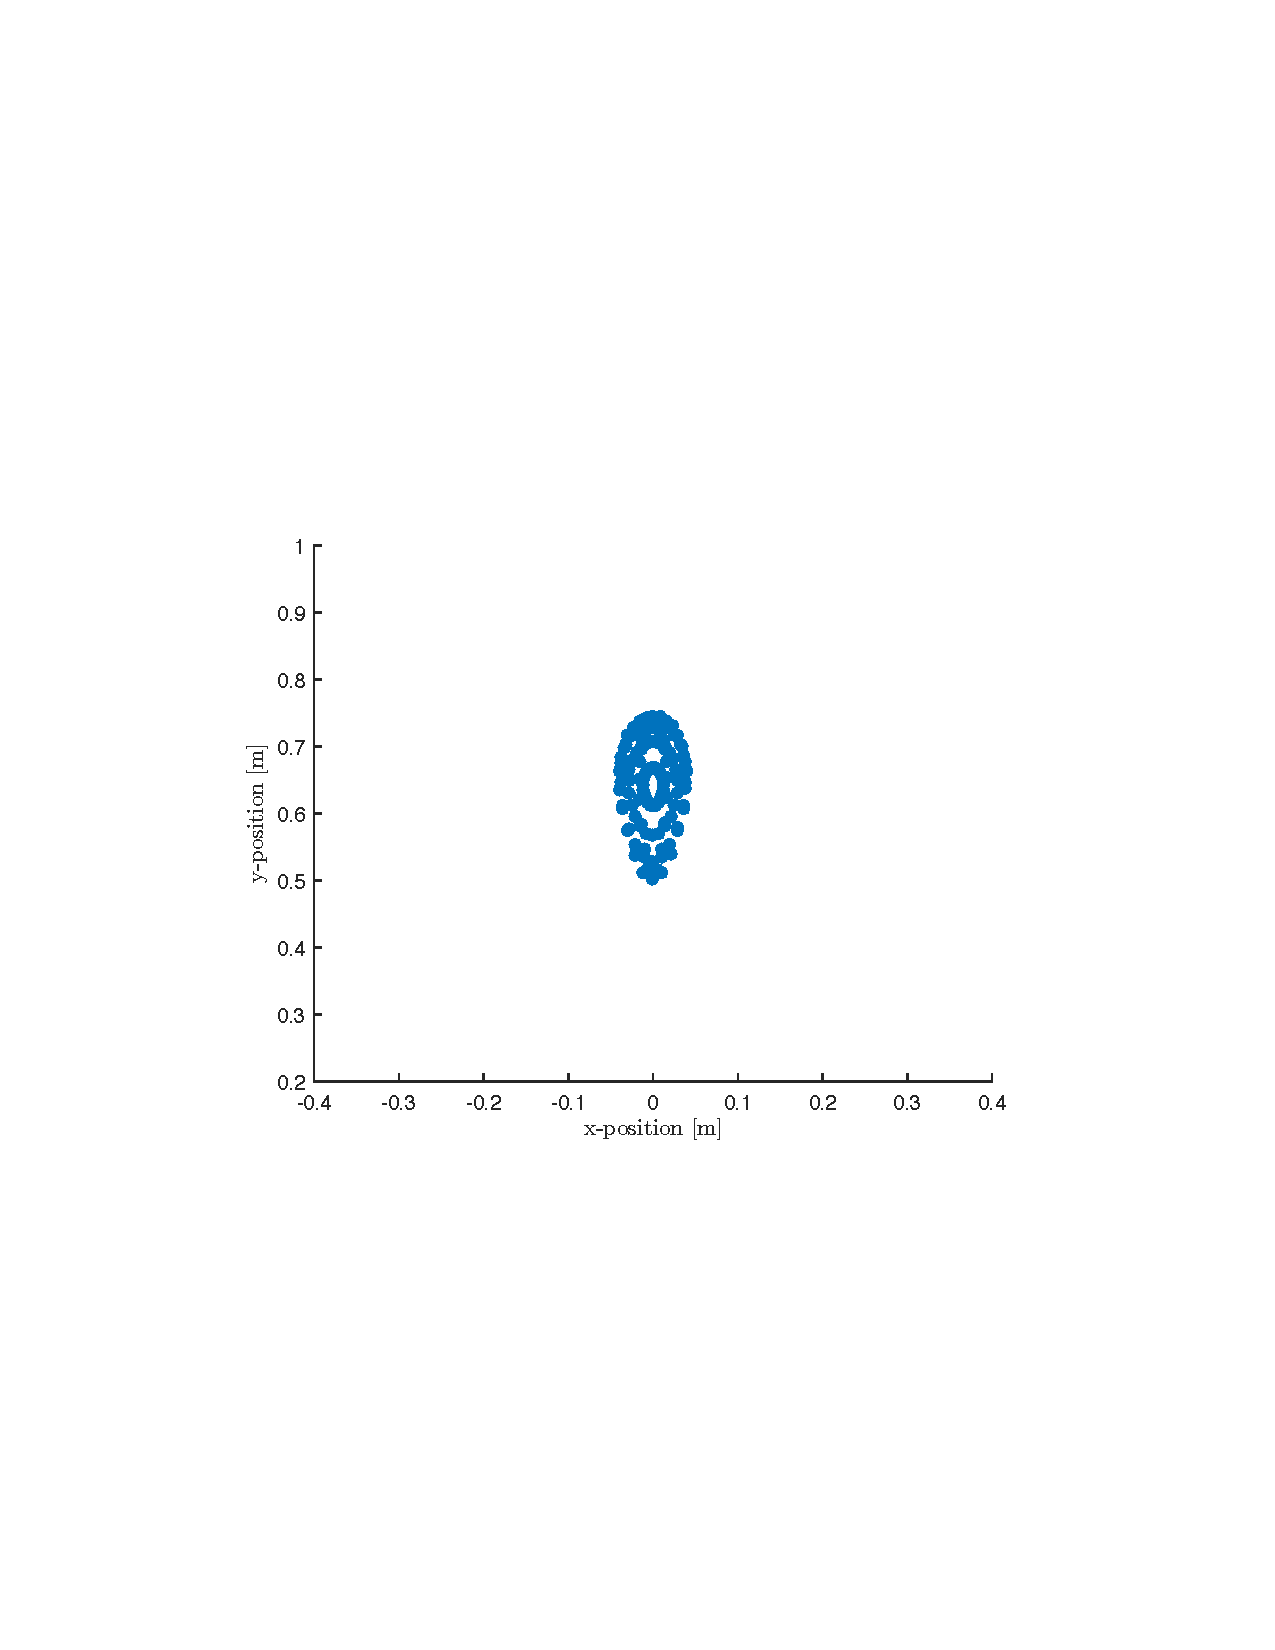
\includegraphics[width=\textwidth]{sh4.pdf}
	\caption{Arc location prediction with a sensor \SI{0.508}{\meter} above the electrode-ingot gap}
	\end{subfigure}
\caption{Arc location prediction trends for varying, single sensor position in the positive z direction with the origin at the sensor location (0,\SI{0.64}{\meter}) using constant furnace coefficients}
\label{fig:trends}
\end{figure}

%%%%%%%%%%%%%%%%%%%%%%%%%%%%%%%%%%%%%%%%%%%%%%%%%%%%
\subsection{Effect of gap size}
\label{sec:gap_size}
%%%%%%%%%%%%%%%%%%%%%%%%%%%%%%%%%%%%%%%%%%%%%%%%%%%%

All previous calculations assumed a constant electrode-ingot gap.
In theory, the gap size should remain approximately constant as the ram raises the electrode based on its melting and solidification rate; in reality, the gap size is constantly changing slightly throughout this process.
This variation could introduce non-negligible errors into the predictions of arc locations, and therefore we studied the effect of gap size on the accuracy of arc location predictions.
Previous studies set the gap height to a constant \SI{0.0254}{\meter}~\cite{Woodside:2010fi,Woodside:2013cf}; here, we varied the height between \numrange{0.5}{2.5} times the baseline value, or specifically \SIlist{0.0127;0.0254;0.0381;0.0635}{\meter}.
Gap sizes considered in the literature include \SI{0.01}{\meter}~\cite{Nair:2009ja,Beaman:2014fi} for smaller radius ingots\slash electrodes, although Zanner studied the effect of gap sizes ranging \SIrange{0.006}{0.05}{\meter}~\cite{Zanner:1984cf} on melt rate.

\begin{figure}[htbp]
	\centering
	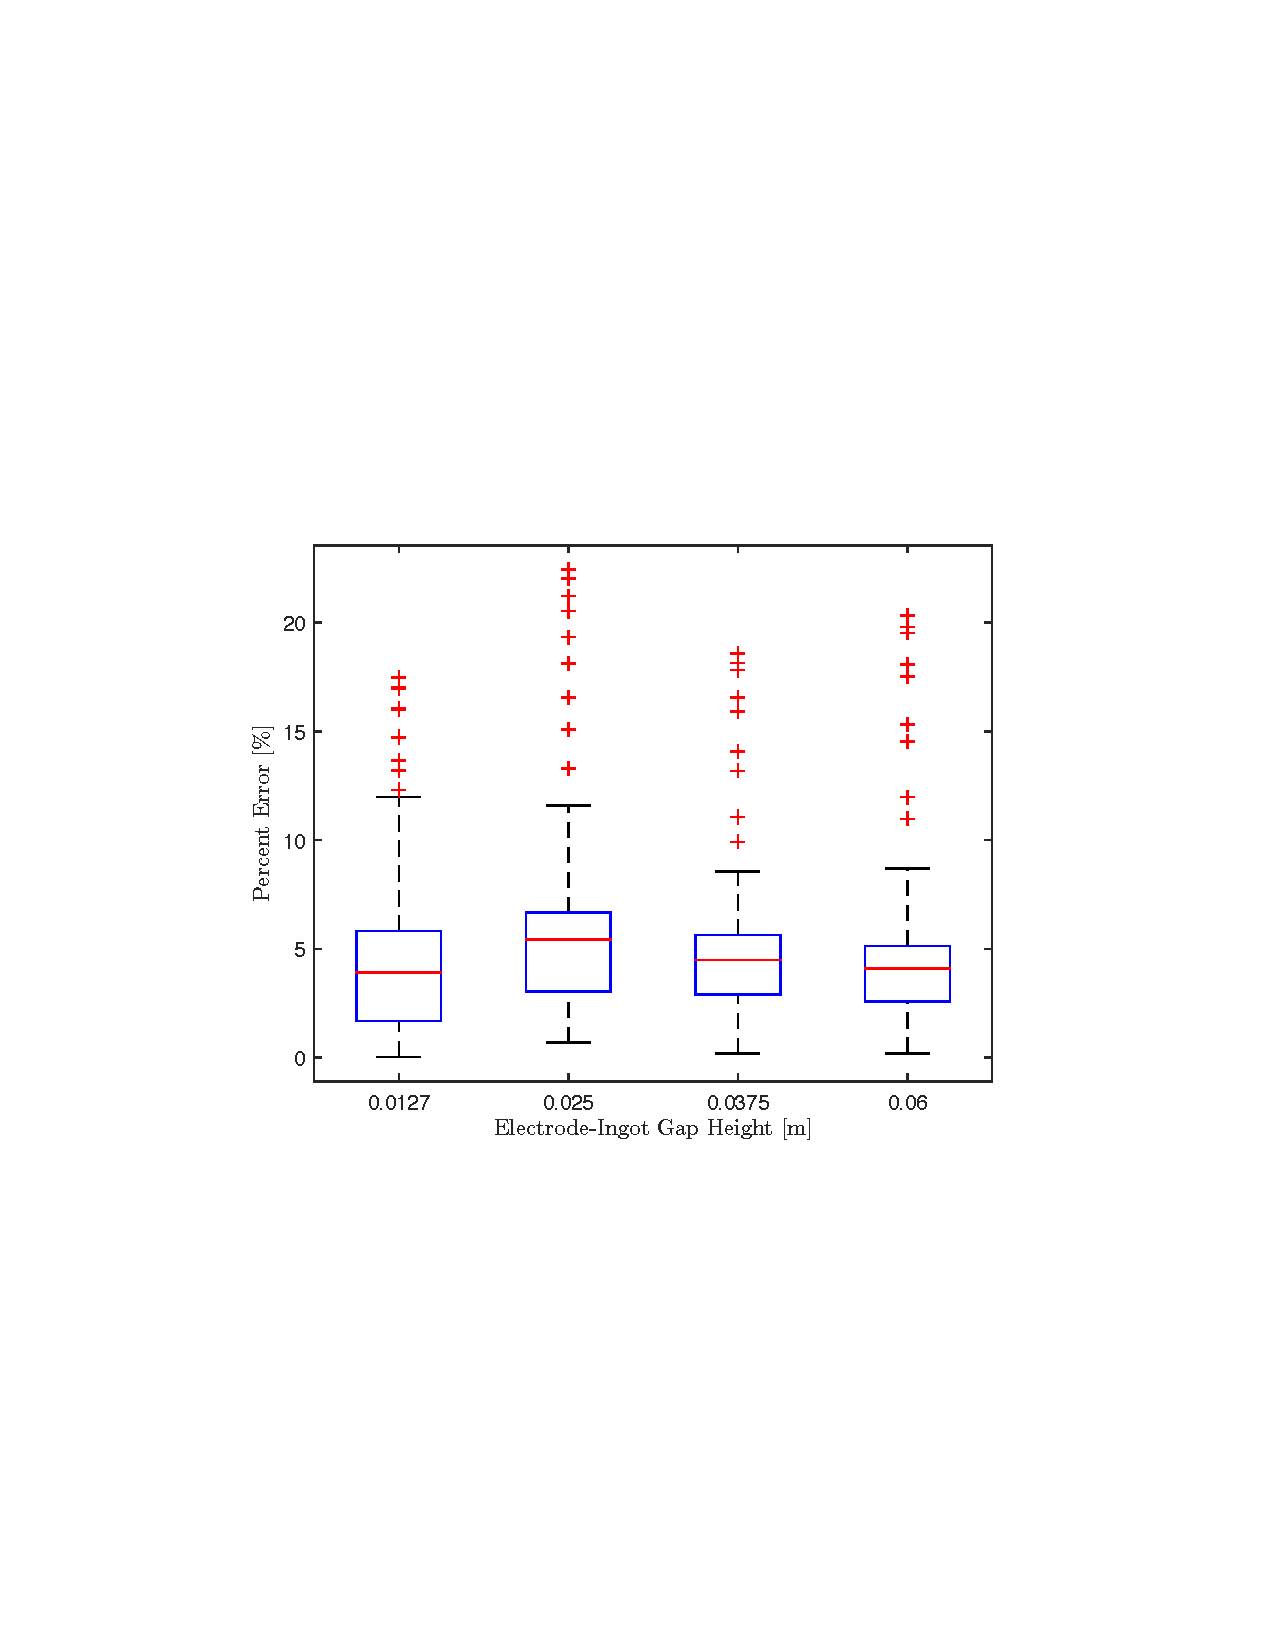
\includegraphics[width=0.6\textwidth]{gap_height_error.pdf}
	\caption{Arc location predictions with varying gap height for a single sensor location}
	\label{fig:compar}
\end{figure}

Figure~\ref{fig:compar} shows arc location predictions with varying gap height for a single sensor location. 
The error in arc location prediction exhibits little sensitivity to gap height; between the smallest and largest gap heights, the median error differs by less than \SI{1.5}{\percent} and the maximum error by less than \SI{5}{\percent}.

%%%%%%%%%%%%%%%%%%%%%%%%%%%%%%%%%%%%%%%%%%%%%%%%%%%%
\subsection{Effect of ingot shrinkage}
\label{sec:shrinkage}
%%%%%%%%%%%%%%%%%%%%%%%%%%%%%%%%%%%%%%%%%%%%%%%%%%%%

The physical characteristics of the ingot differ drastically from top to bottom during the melting process.
At the top, a molten pool of liquid metal circulates on top of the soft, hot metal solidifying near the sides and bottom. 
As the VAR process continues and the ingot grows, the metal cools and contracts.
This causes the metal to shrink and pull away from the crucible, reducing the electrical contact surface area with the crucible; this behavior is known as ingot shrinkage.
The section of the material that remains in contact with the crucible wall is called the contact zone.
Since shrinkage changes the surface area of the ingot that contacts the crucible wall---and thus the area where electrical current passes---it could alter the current path and thus the magnetic field distribution, potentially affecting predictions of arc location.
We studied the effects of shrinkage by applying grounded boundary conditions to the contact zone and electrical insulation to the shrinkage gap zone, following the approach of Pericleous et al.~\cite{Pericleous:2013kb}.
We varied the size of the contact zone from the full length of the ingot to \SI{0.032}{\meter}, ranging from zero shrinkage to a contact zone \SI{3}{\percent} of the ingot height.

\begin{figure}[htbp]
\centering
	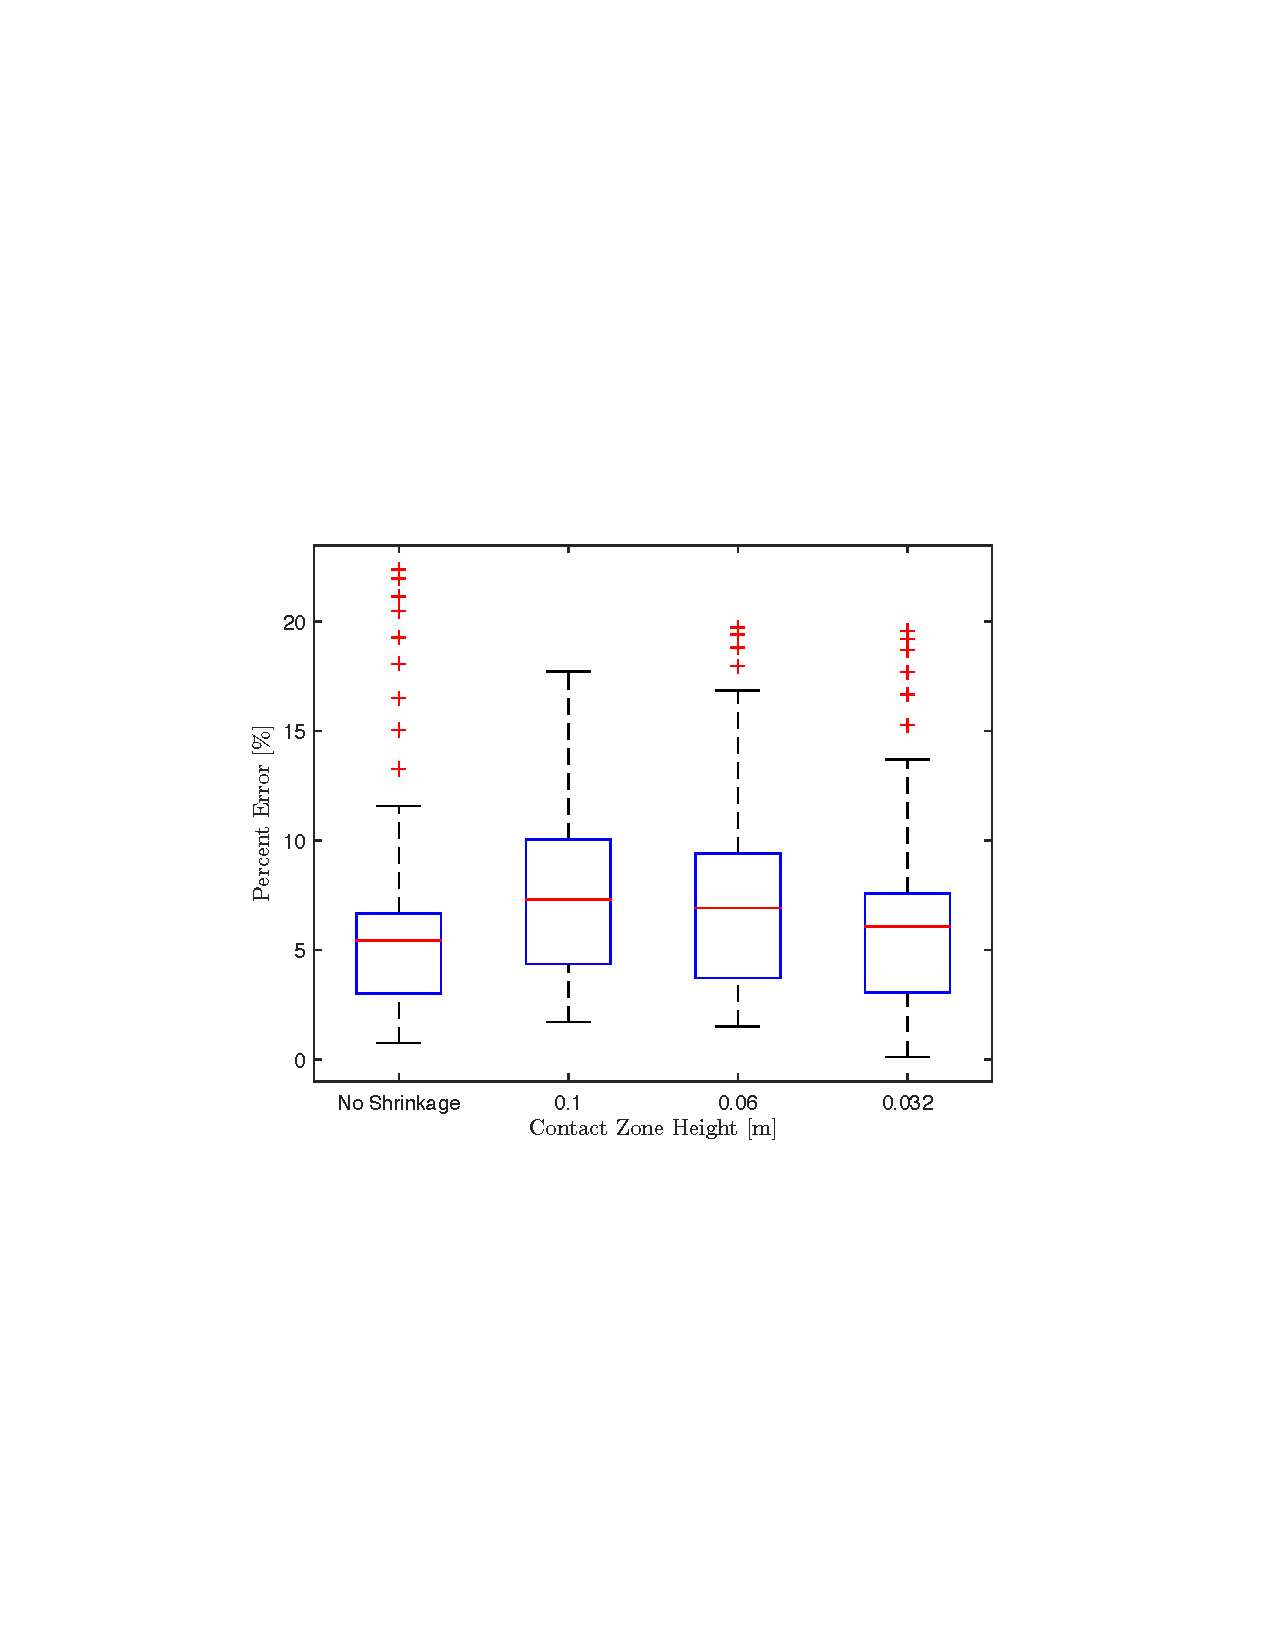
\includegraphics[width=0.6\textwidth]{shrinkage_study_error.pdf}
	\caption{Error in predicted arc locations with varying contact zone height, mimicking ingot shrinkage}
	\label{fig:shrinkage}
\end{figure}

Figure~\ref{fig:shrinkage} shows the error distribution for predicted arc locations with increasing shrinkage, corresponding to decreasing contact zone height.
While error increases slightly as the contact zone shrinks, in general shrinkage causes an median error increase of less than \SI{2}{\percent} in predicted arc locations, corresponding to a similar change in magnetic flux density.
However, the higher current density resulting from smaller contact zones could affect the $z$ component of magnetic flux density more significantly---although this component does not play a role in the current APS approach based on horizontal (i.e., $x$ and $y$) components.

%%%%%%%%%%%%%%%%%%%%%%%%%%%%%%%%%%%%%%%%%%%%%%%%%%%%
\subsection{Effect of using multiple sensors}
\label{sec:multiple_sensors}
%%%%%%%%%%%%%%%%%%%%%%%%%%%%%%%%%%%%%%%%%%%%%%%%%%%%

Thus far, we only used magnetic field measurements at one sensor location for calculations to determine arc locations. 
Both our results and those from Woodside et al.~\cite{Woodside:2010fi,Woodside:2013cf} show that the error increases as the arc moves away from the sensor. 
Therefore, for an axisymmetric system, we hypothesize that the results from multiple sensors can be averaged to improve the accuracy of the overall prediction.
To test this, we averaged predicted arc locations from \numrange{2}{16} evenly spaced sensors around the furnace.

First, we examined the trends in arc location prediction for two separate sensors located at opposite sides of the furnace; Figure~\ref{fig:two_sensors} shows these (separate) predicted arc locations, compared with the exact locations.
Although the sensors predict similar locations for arcs located near the center of the furnace, near the perimeters the predicted locations exhibit a bias towards the closer sensor.
Figure~\ref{fig:4ave} compares exact arc locations with predictions based on the average location from four evenly spaced sensors.
The averaging resulted in an even spacial distribution of the arc positions; as Figure~\ref{fig:4error} shows, the error predicted locations is also evenly distributed compared with that from a single sensor.
This information is useful because it can be used to develop correction algorithms to predict arc locations more accurately.
Based on these results, more sensors might aid in smoothing the error further; however, evenly distributed results do not guarantee more accurate results---in fact, outliers could bias the predictions.
Figure~\ref{fig:numsens} shows the error distribution in predicted arc locations achieved by averaging calculations using \numlist{1;2;4;8;16} evenly distributed sensors.
The error distribution contracts with the addition of sensors, but the predictions do not improve with more than four sensors.

Now we can analyze whether using four sensor averaging of arc location predictions aid in the reduction of error for a varying sensor height.
In Section~\ref{sec:vertical_position} we calculated how error distribution was affected by the relative vertical position of a single sensor with respect to the electrode-ingot gap. 
Now, we apply the same methodology while using arc location predictions determined with four-sensor averaging. 
The results are shown in Figure~\ref{fig:fourheight}. 
The total error distribution is smaller than the single-sensor results from Section~\ref{sec:vertical_position} with a maximum error of less than \SI{16}{\percent} at the highest and lowest positions. 
Using four sensors also suppresses the outliers.
These results were calculated using varying furnace coefficients; the coefficients were recalculated at every vertical position.

\begin{figure}[htbp]
\centering
	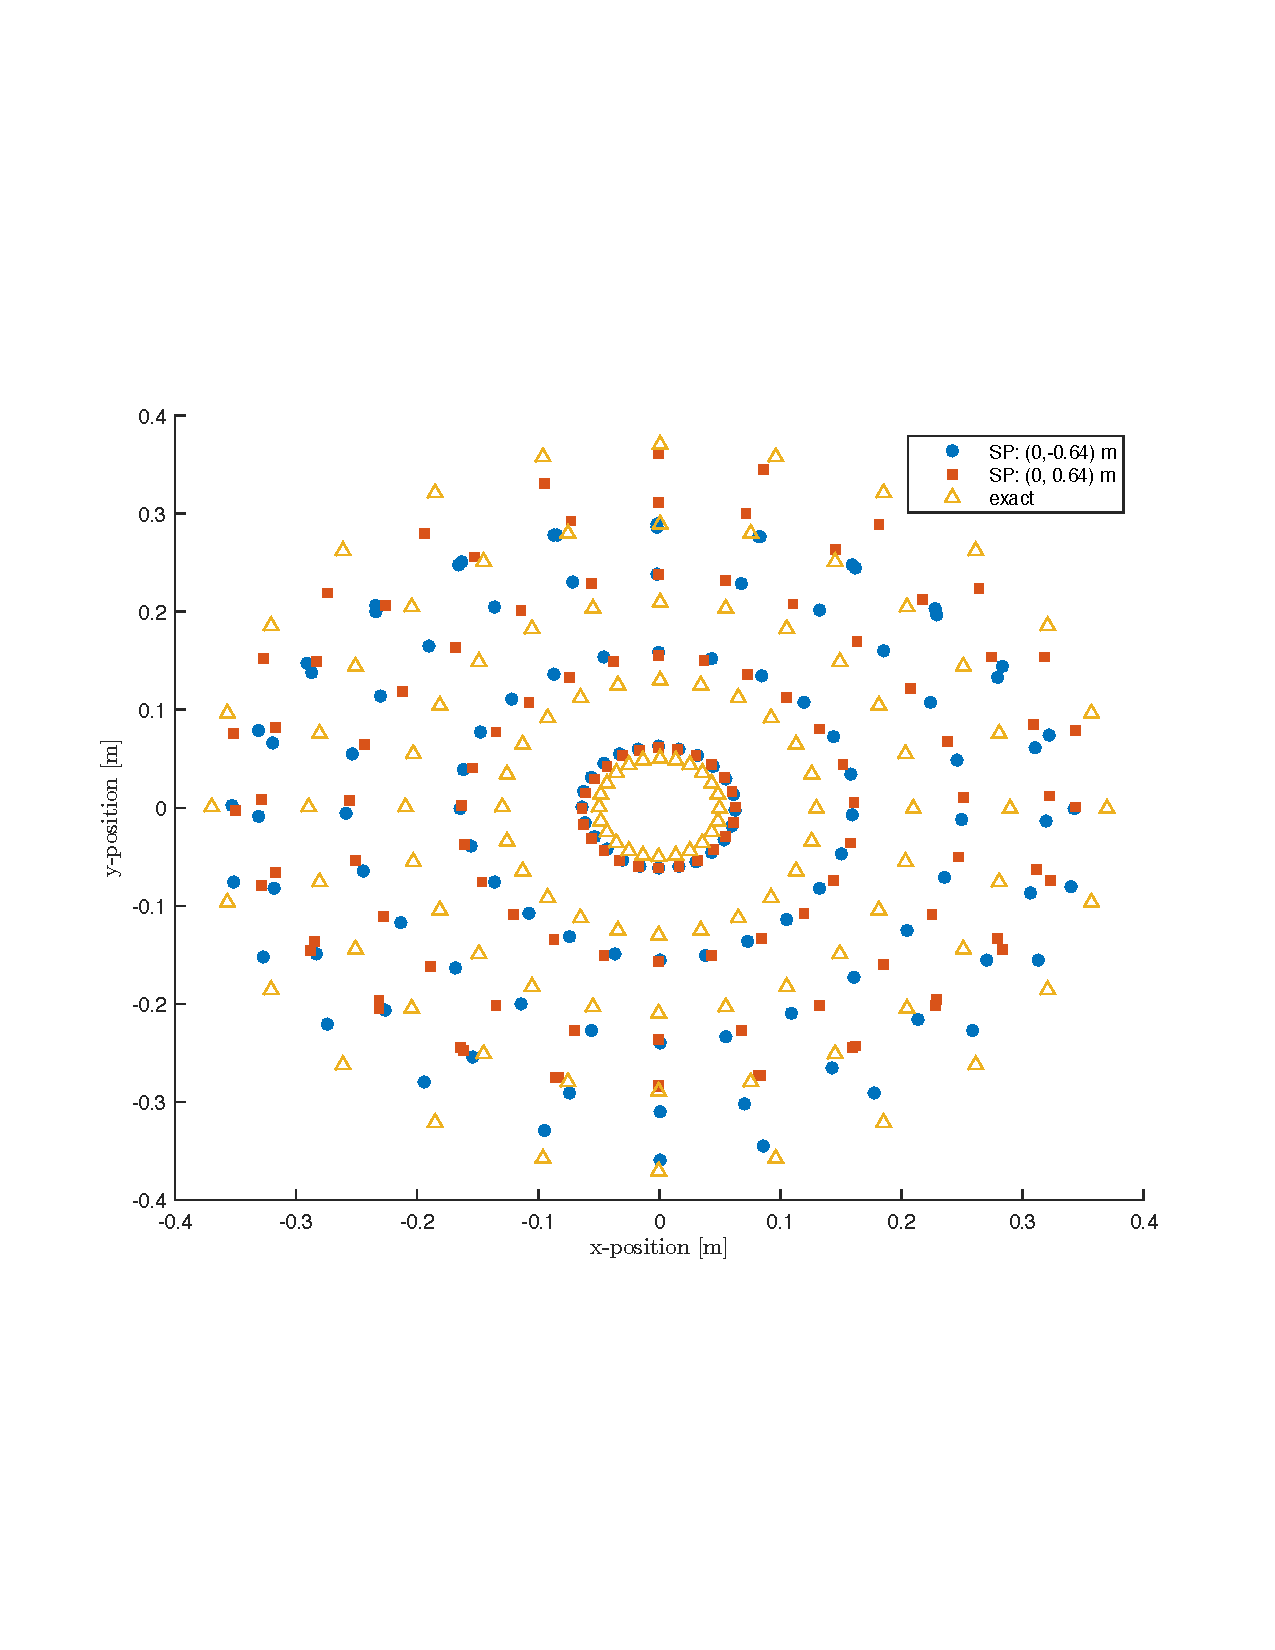
\includegraphics[width=0.6\textwidth]{senspos.pdf}
	\caption{Arc location predictions for two sensors position on opposite sides of the furnace: (\SI{0}{\meter}, \SI{-0.64}{\meter}) and (\SI{0}{\meter}, \SI{0.64}{\meter})}
	\label{fig:two_sensors}
\end{figure}

\begin{figure}[htbp]
\centering
	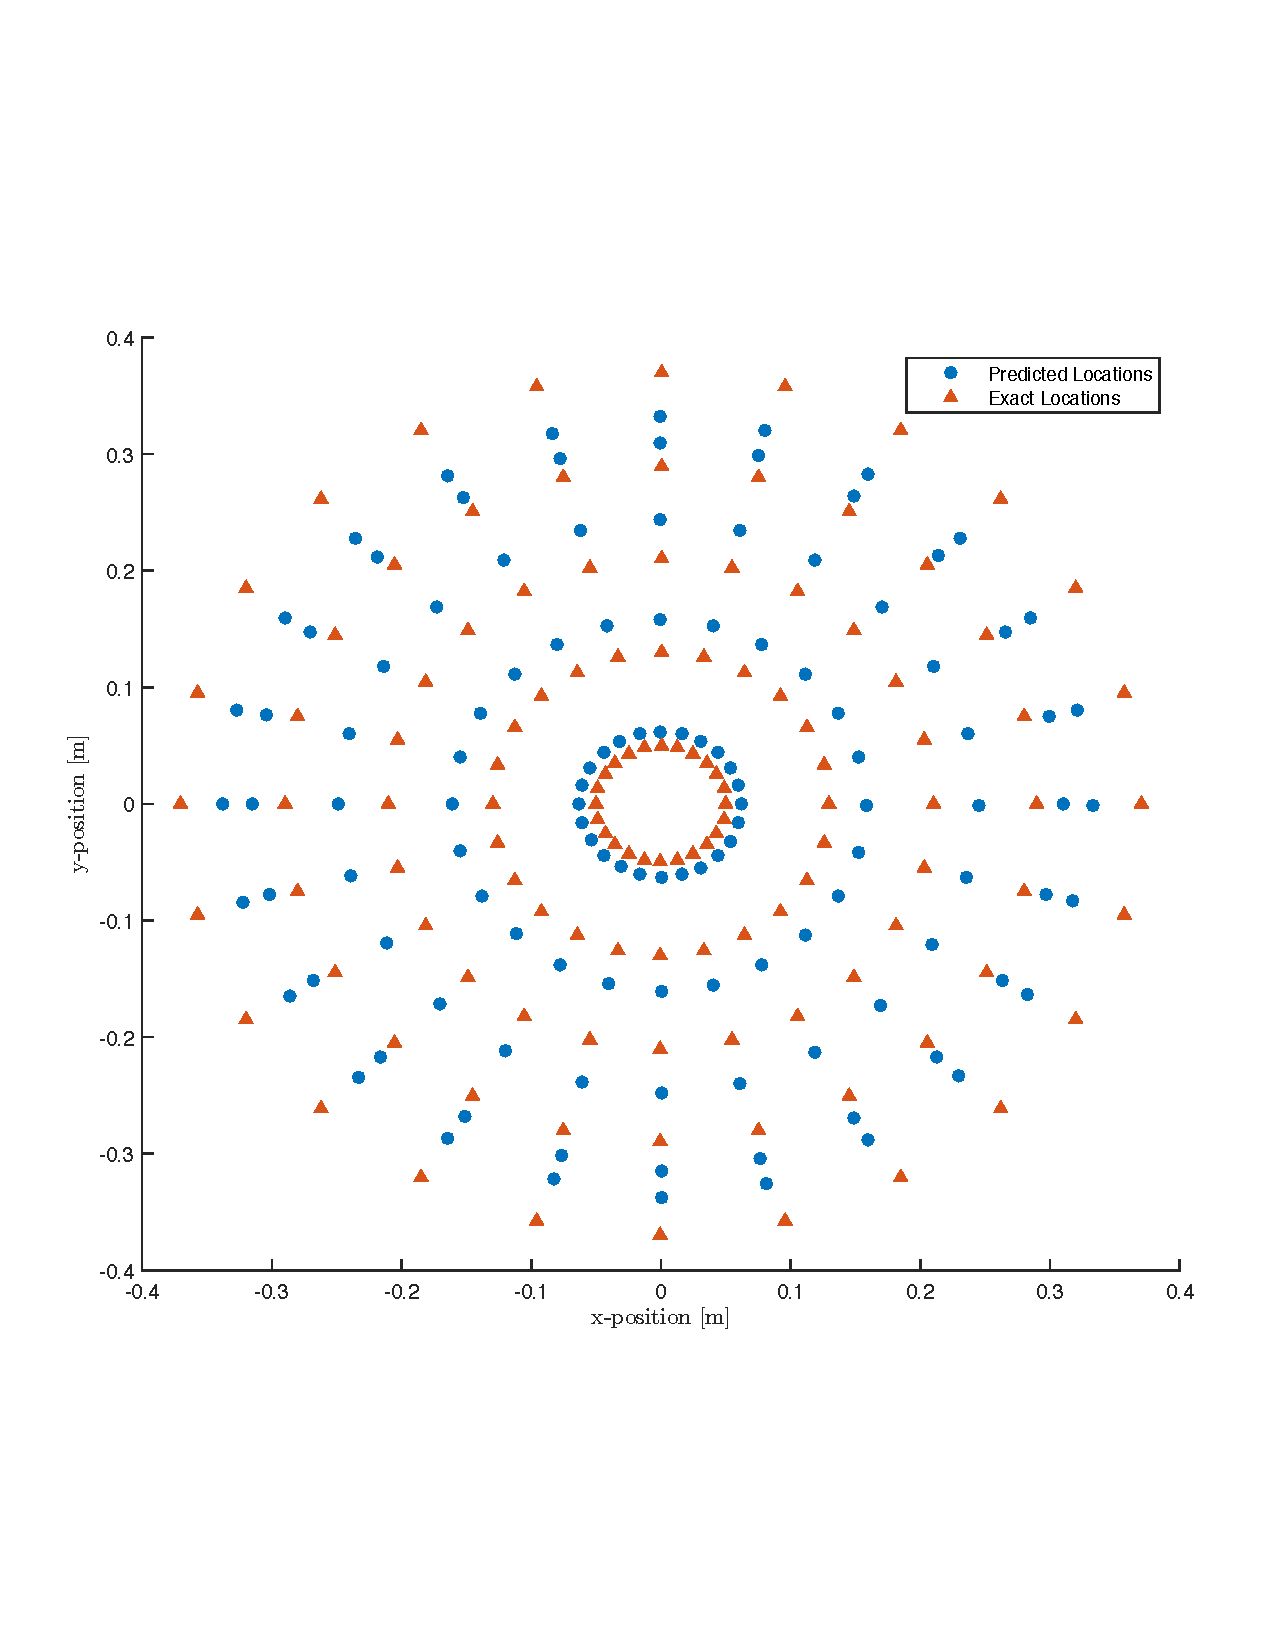
\includegraphics[width=0.6\textwidth]{foursenspred.pdf}
	\caption{Arc location predictions using four sensors around the furnace; these locations are the average of the locations predicted by each of the four sensors}
	\label{fig:4ave}
\end{figure}


\begin{figure}[htbp]
	\centering
	\begin{subfigure}[b]{0.495\textwidth}
	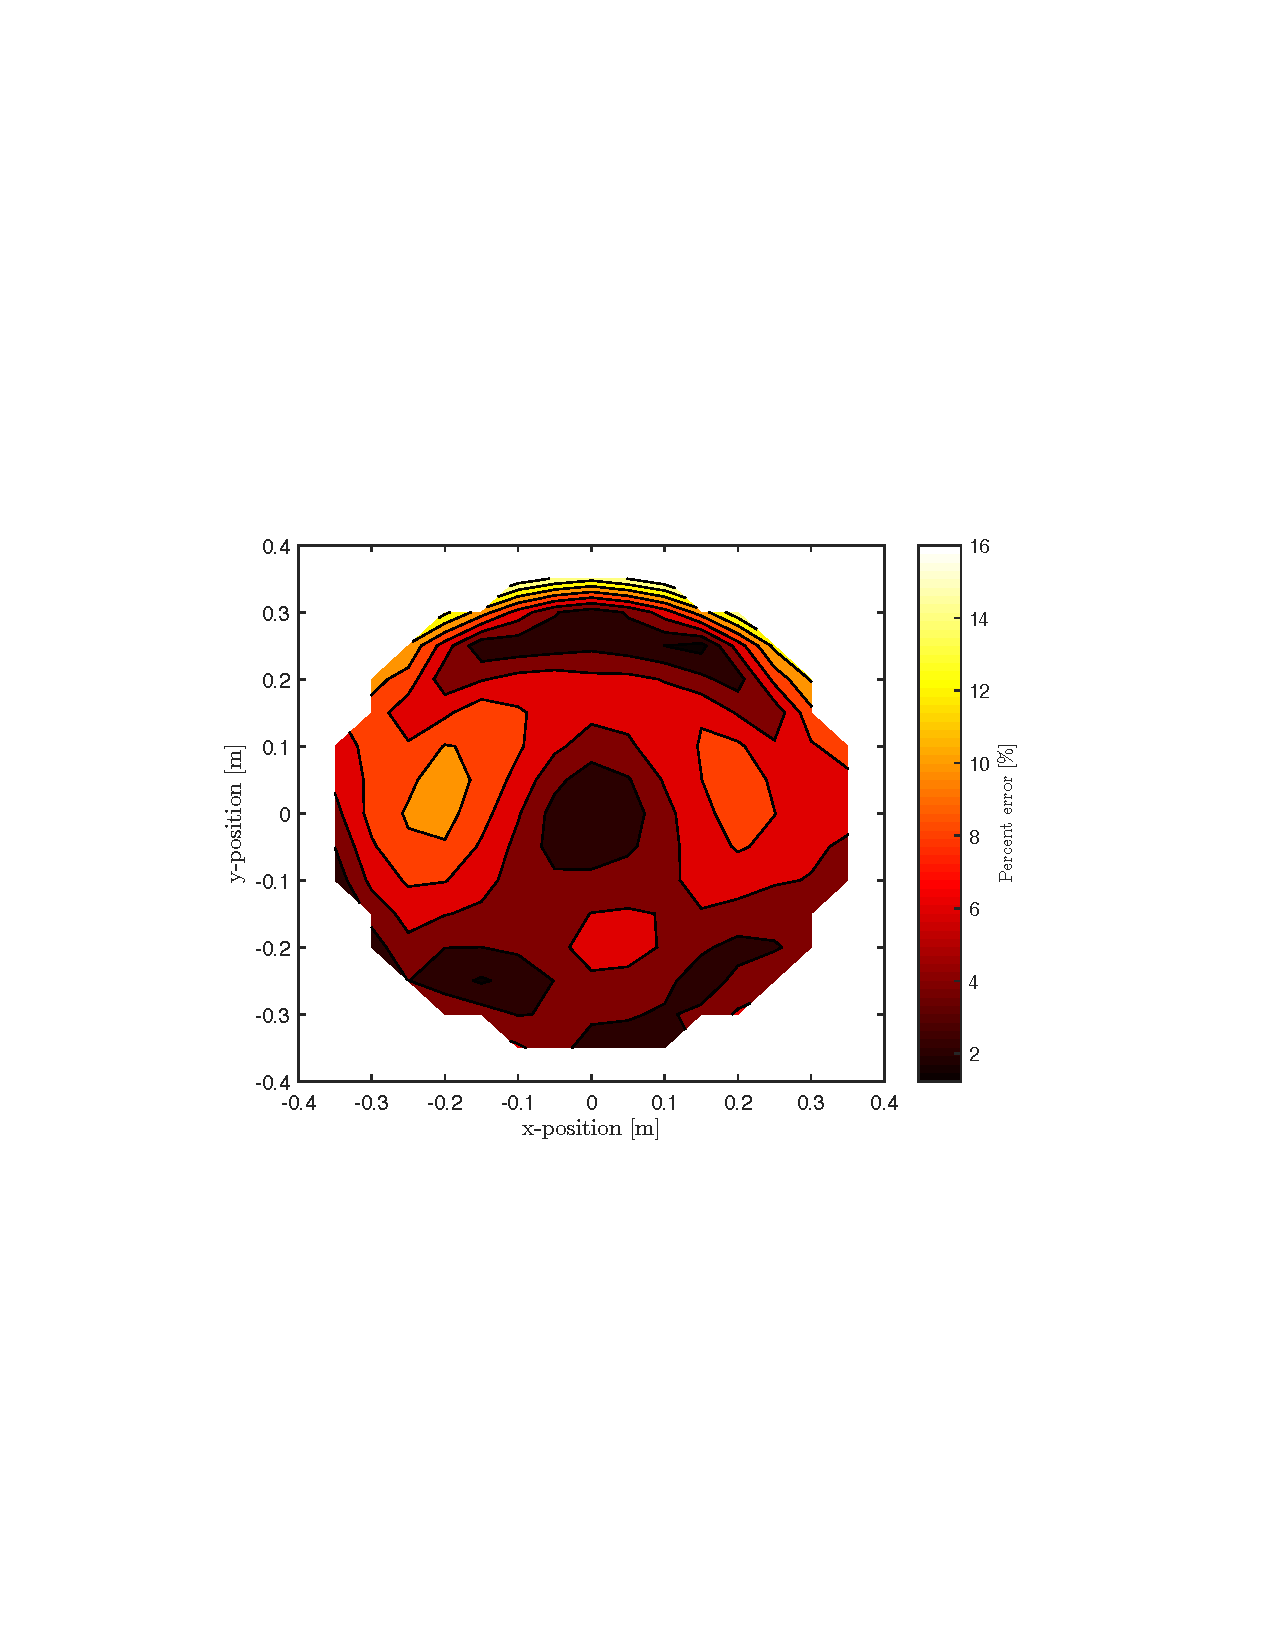
\includegraphics[width=\textwidth]{one_sensor_percent_error_contour.pdf}
	\caption{Percent error of arc location predictions using one sensor from the exact locations}
		\label{fig:1error}
	\end{subfigure}
	\hfill
	\begin{subfigure}[b]{0.495\textwidth}
	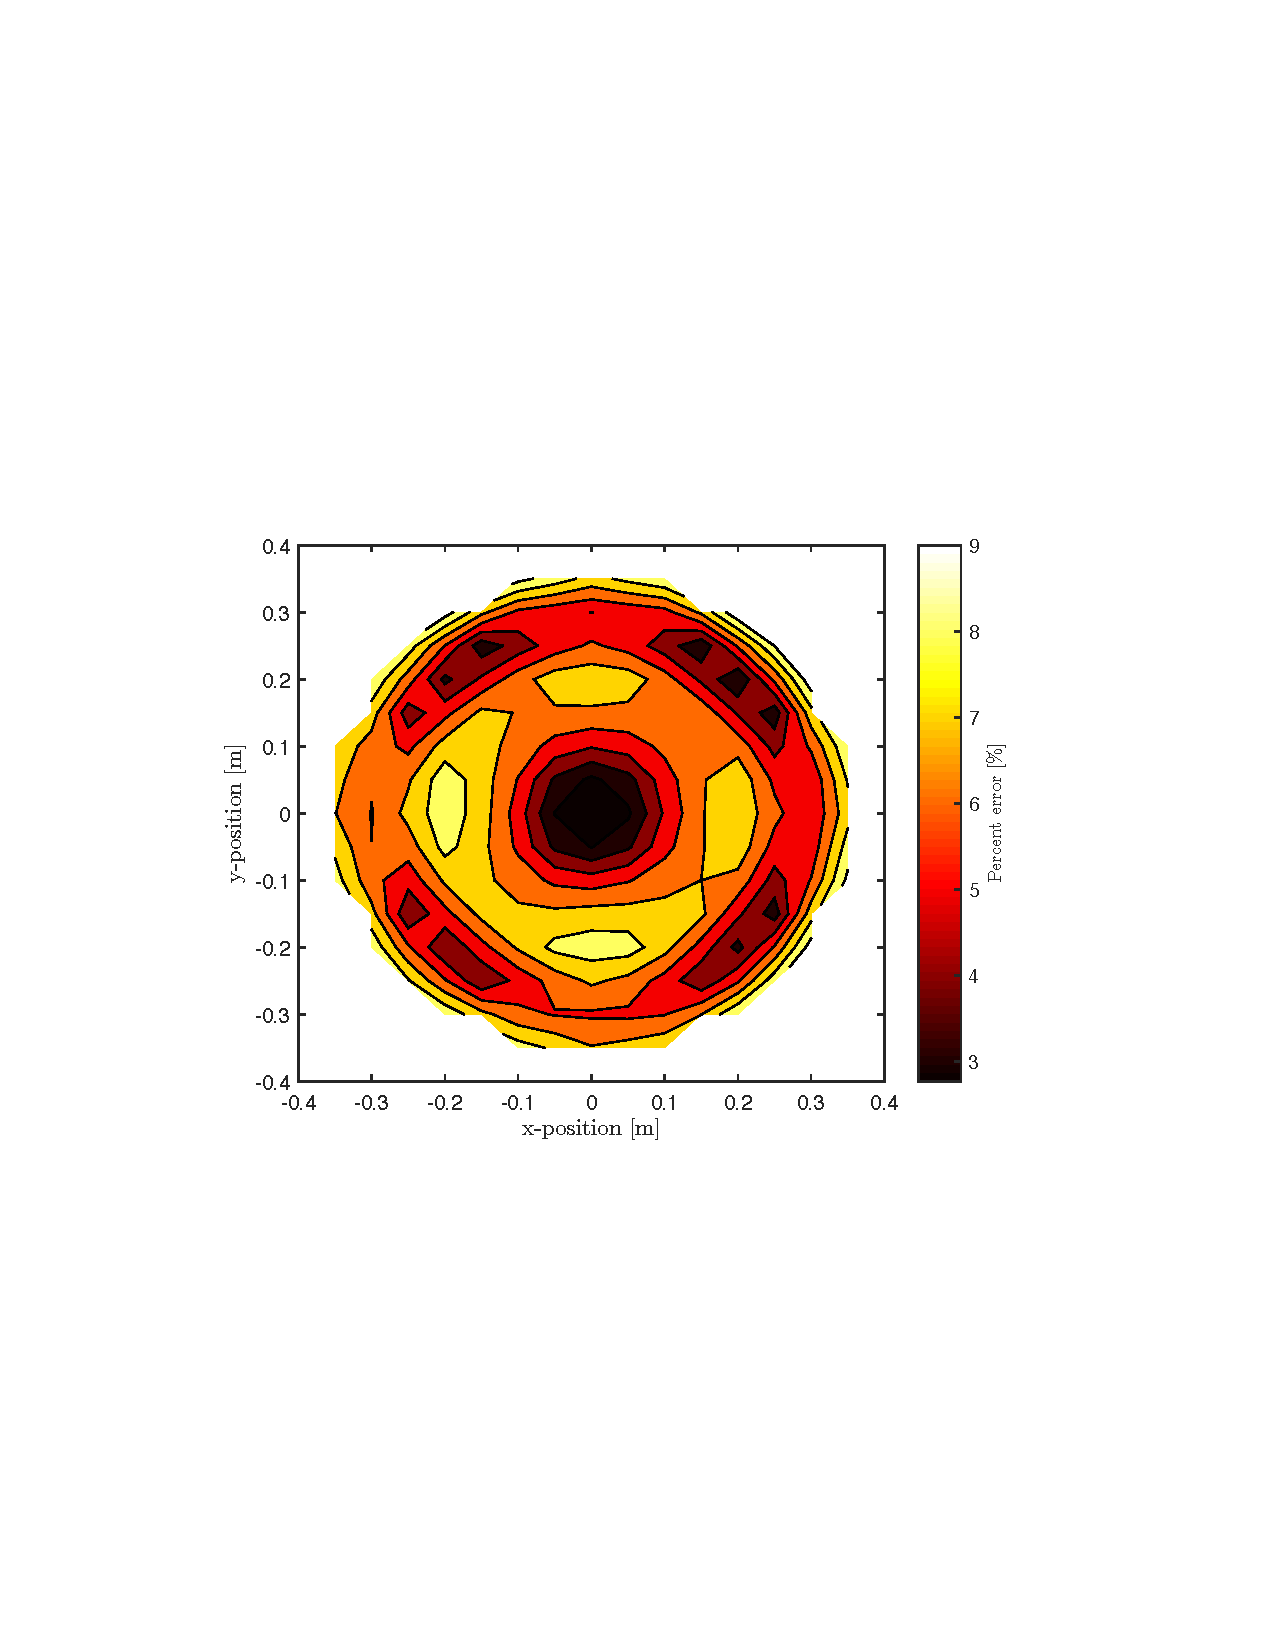
\includegraphics[width=\textwidth]{four_sensor_percent_error_contour.pdf}
	\caption{Percent error of arc location predictions using four sensor averaging from the exact locations}
	\end{subfigure}
	\caption{Comparison of error distribution and magnitude from using one sensor versus four sensor averages; error is based on difference between predicted and exact values}
	\label{fig:4error}
\end{figure}

\begin{figure}[htbp]
\centering
	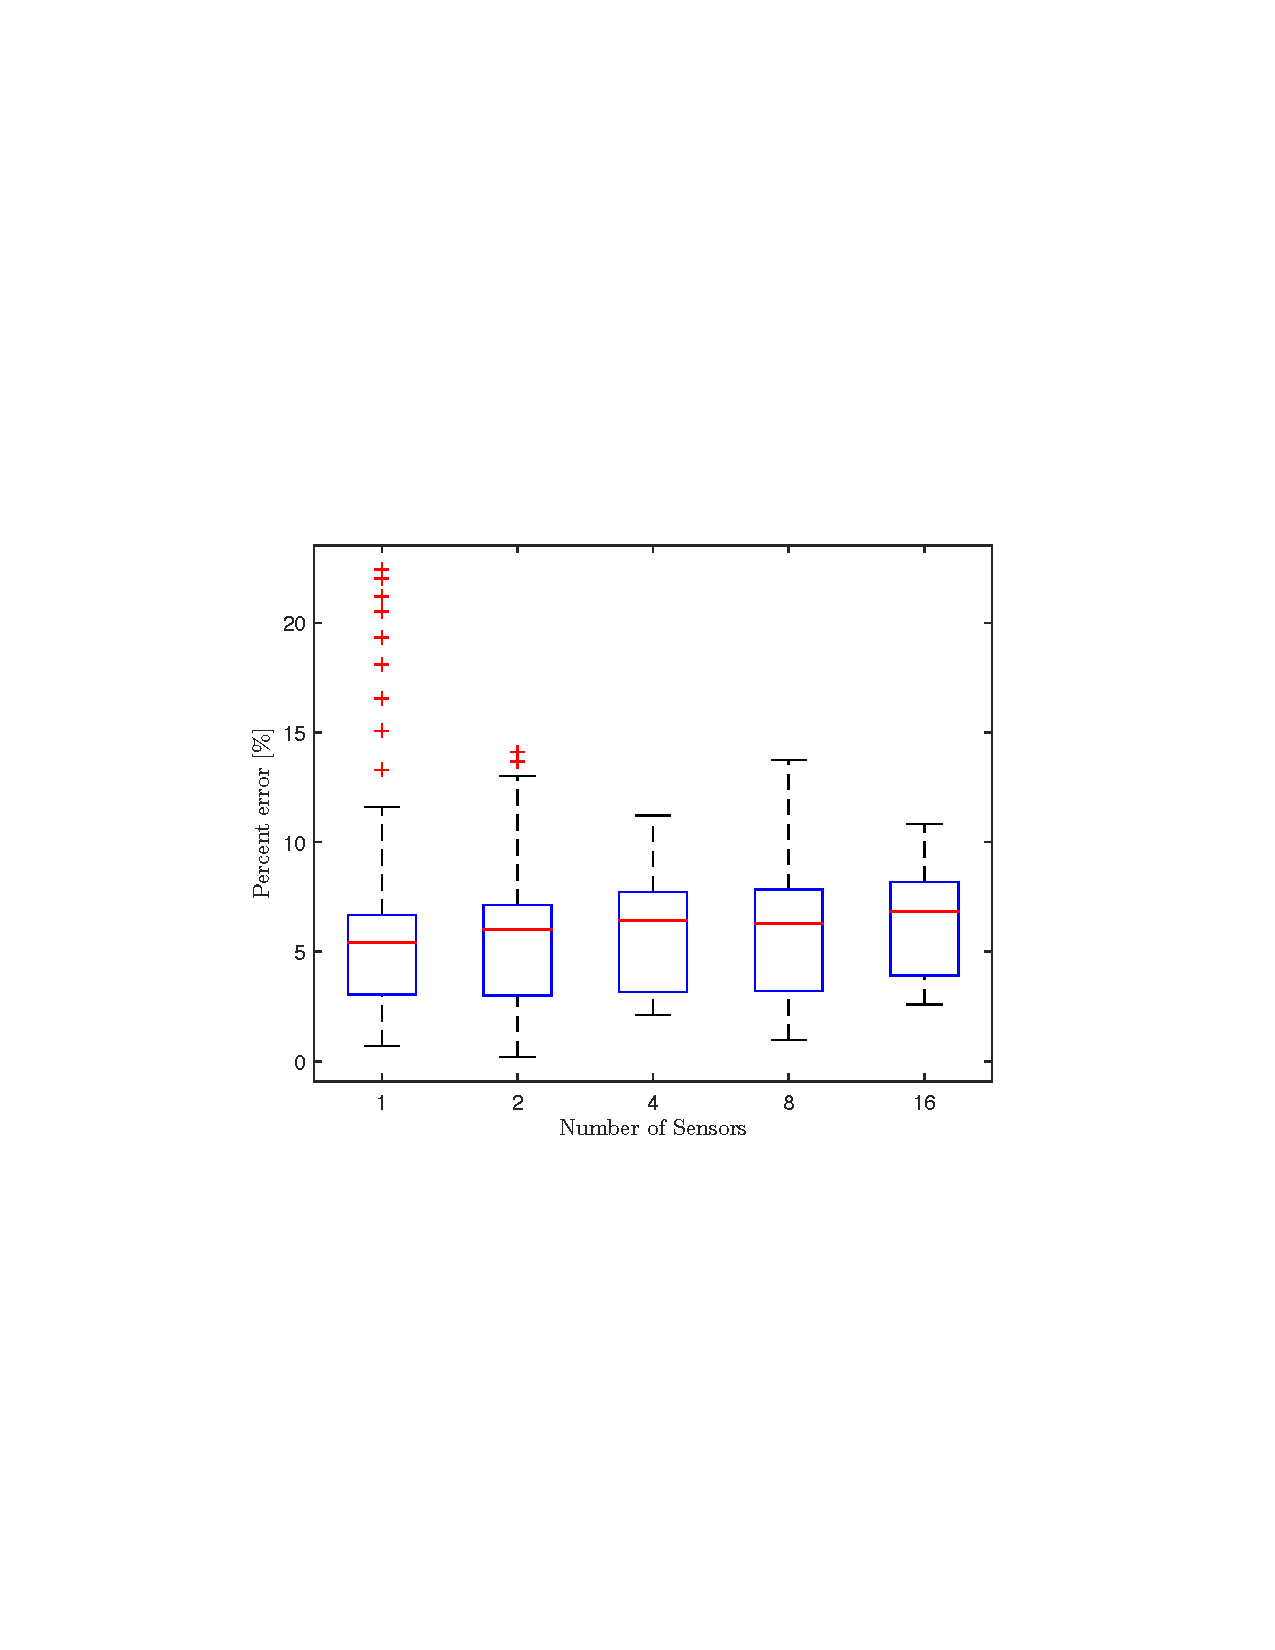
\includegraphics[width=0.6\textwidth]{num_sens_opt_error.pdf}
	\caption{Percent error statistical distribution for 1, 2, 4, 8, and 16 sensors}
	\label{fig:numsens}
\end{figure}

\begin{figure}[htbp]
\centering
	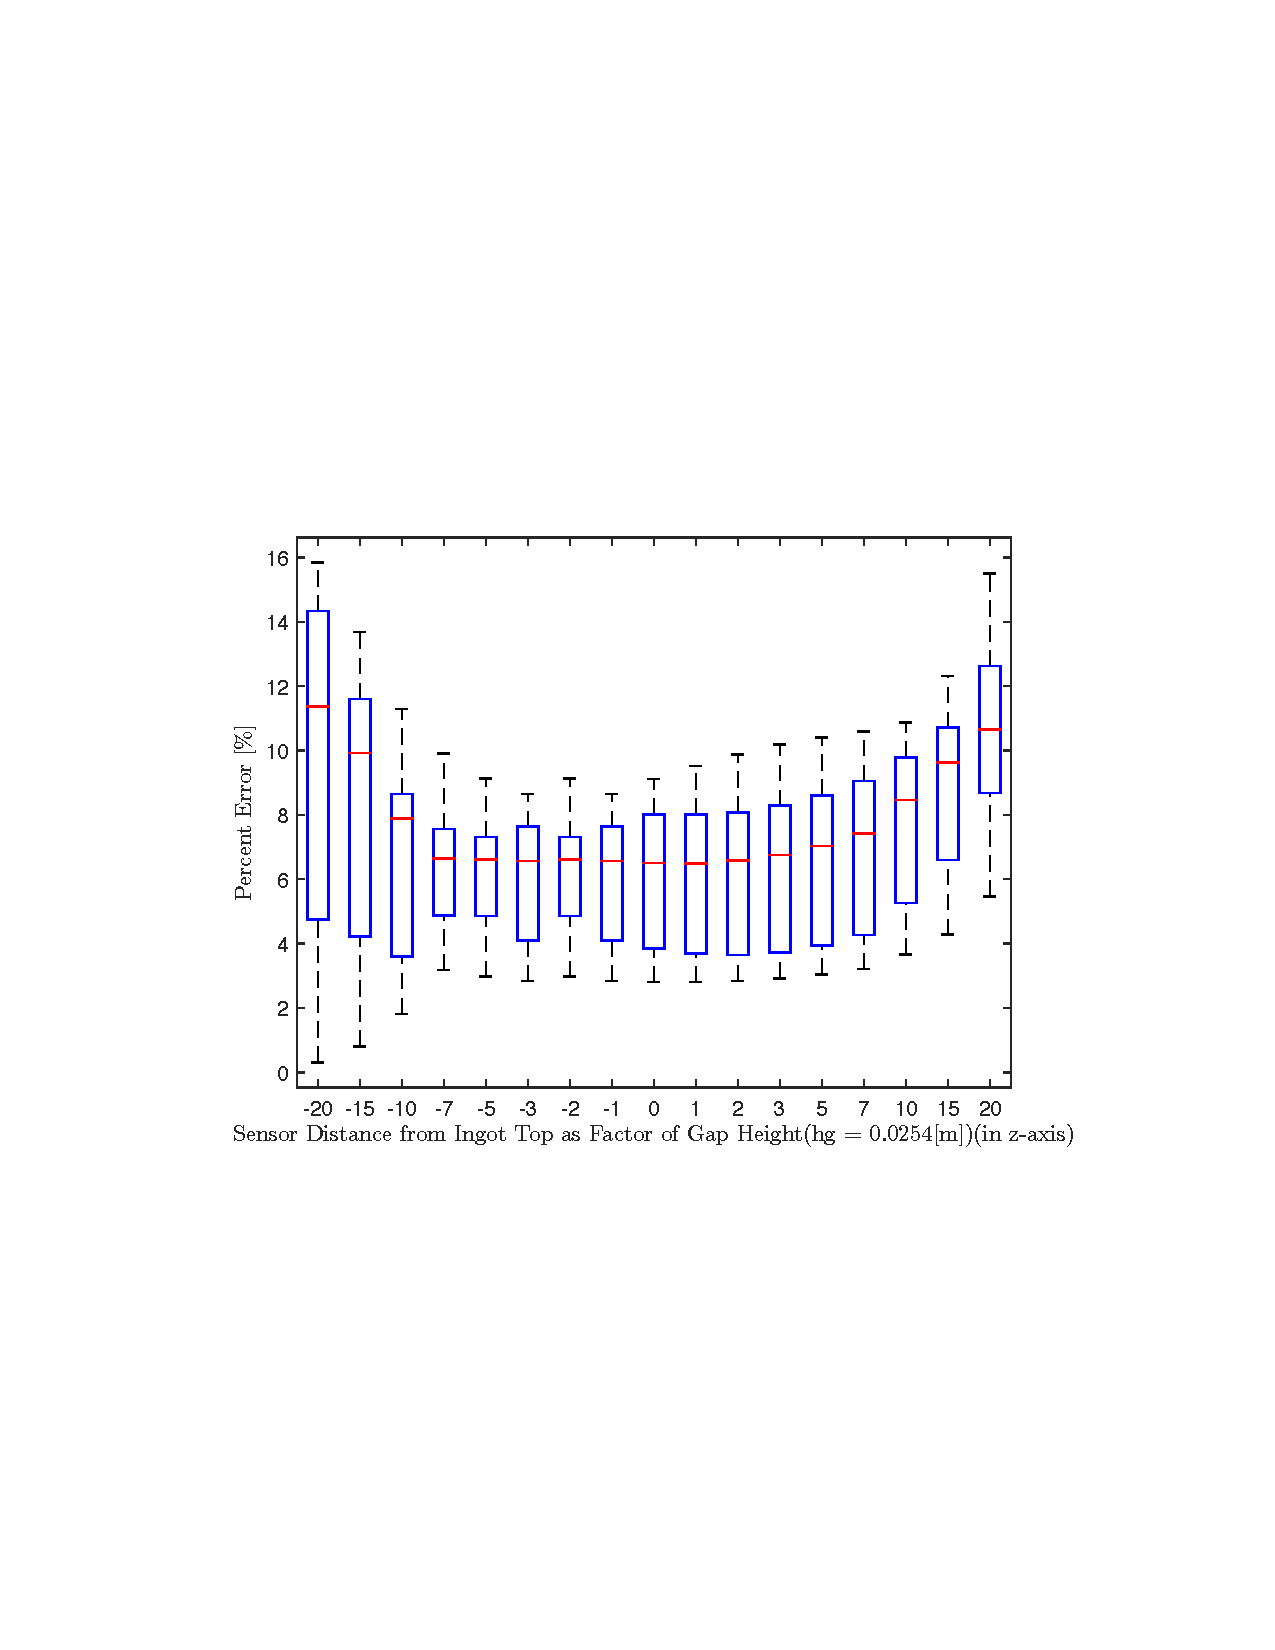
\includegraphics[width=0.6\textwidth]{four_sensor_sens_height.pdf}
	\caption{Error distribution of predicted arc locations with respect to vertical sensor position using the average results from four sensors}
	\label{fig:fourheight}
\end{figure}


%%%%%%%%%%%%%%%%%%%%%%%%%%%%%%%%%%%%%%%%%%%%%%%%%%%%
%\subsection{Exploration of metal-vapor plasma in gap}
%%%%%%%%%%%%%%%%%%%%%%%%%%%%%%%%%%%%%%%%%%%%%%%%%%%%

%During a real VAR process, the vacuum chamber does not remain under a vacuum.
%Instead, a metal-vapor plasma forms due to loss of electrons caused by the action of the arc(s) on the electrode.
%This plasma generation impacts the results because it alters the arc current distribution, and therefore magnetic field strength.~\cite{Wang:2005fg,Pericleous:2013kb}.
%Figure~\ref{fig:currentsens} shows the fraction of current in the arc, relative to the total input current to the system, as a function of the conductivity of material in the ``vacuum'' space (i.e., the electrode-ingot gap).
%A three order-of-magnitude increase in conductivity of the gap material reduces the fraction of current passing through the arc by a factor of 10, and additional increases in conductivity further reduce this fraction.
%The current density in the arc plays a strong role in the prediction of arc locations, as indicated in Eqs.~\eqref{eq:magnetic_t} and \eqref{eq:magnetic_r}.
%Thus, Fig.~\ref{fig:currentsens} reveals that the model is sensitive to the conductivity of the simulated metal-vapor plasma.
%Our approach to modeling the arc requires a substantial fraction of the current density to travel through the arc.
%Increasing the fraction of ``vacuum'' conductivity to arc conductivity from $10^{-5}$ to $10^{-3}$ results in the collapse of the methodology. 
%However, these conductivity values for the plasma may even be unrealistically low, since plasma is actually highly conductive.
%Without better estimates---or a better physics-based approach to modeling the arc and metal-vapor plasma---we cannot state with certainty the level of impact the metal-vapor plasma has on predictions of arc location.

%\begin{figure}[htbp]
%\centering
%	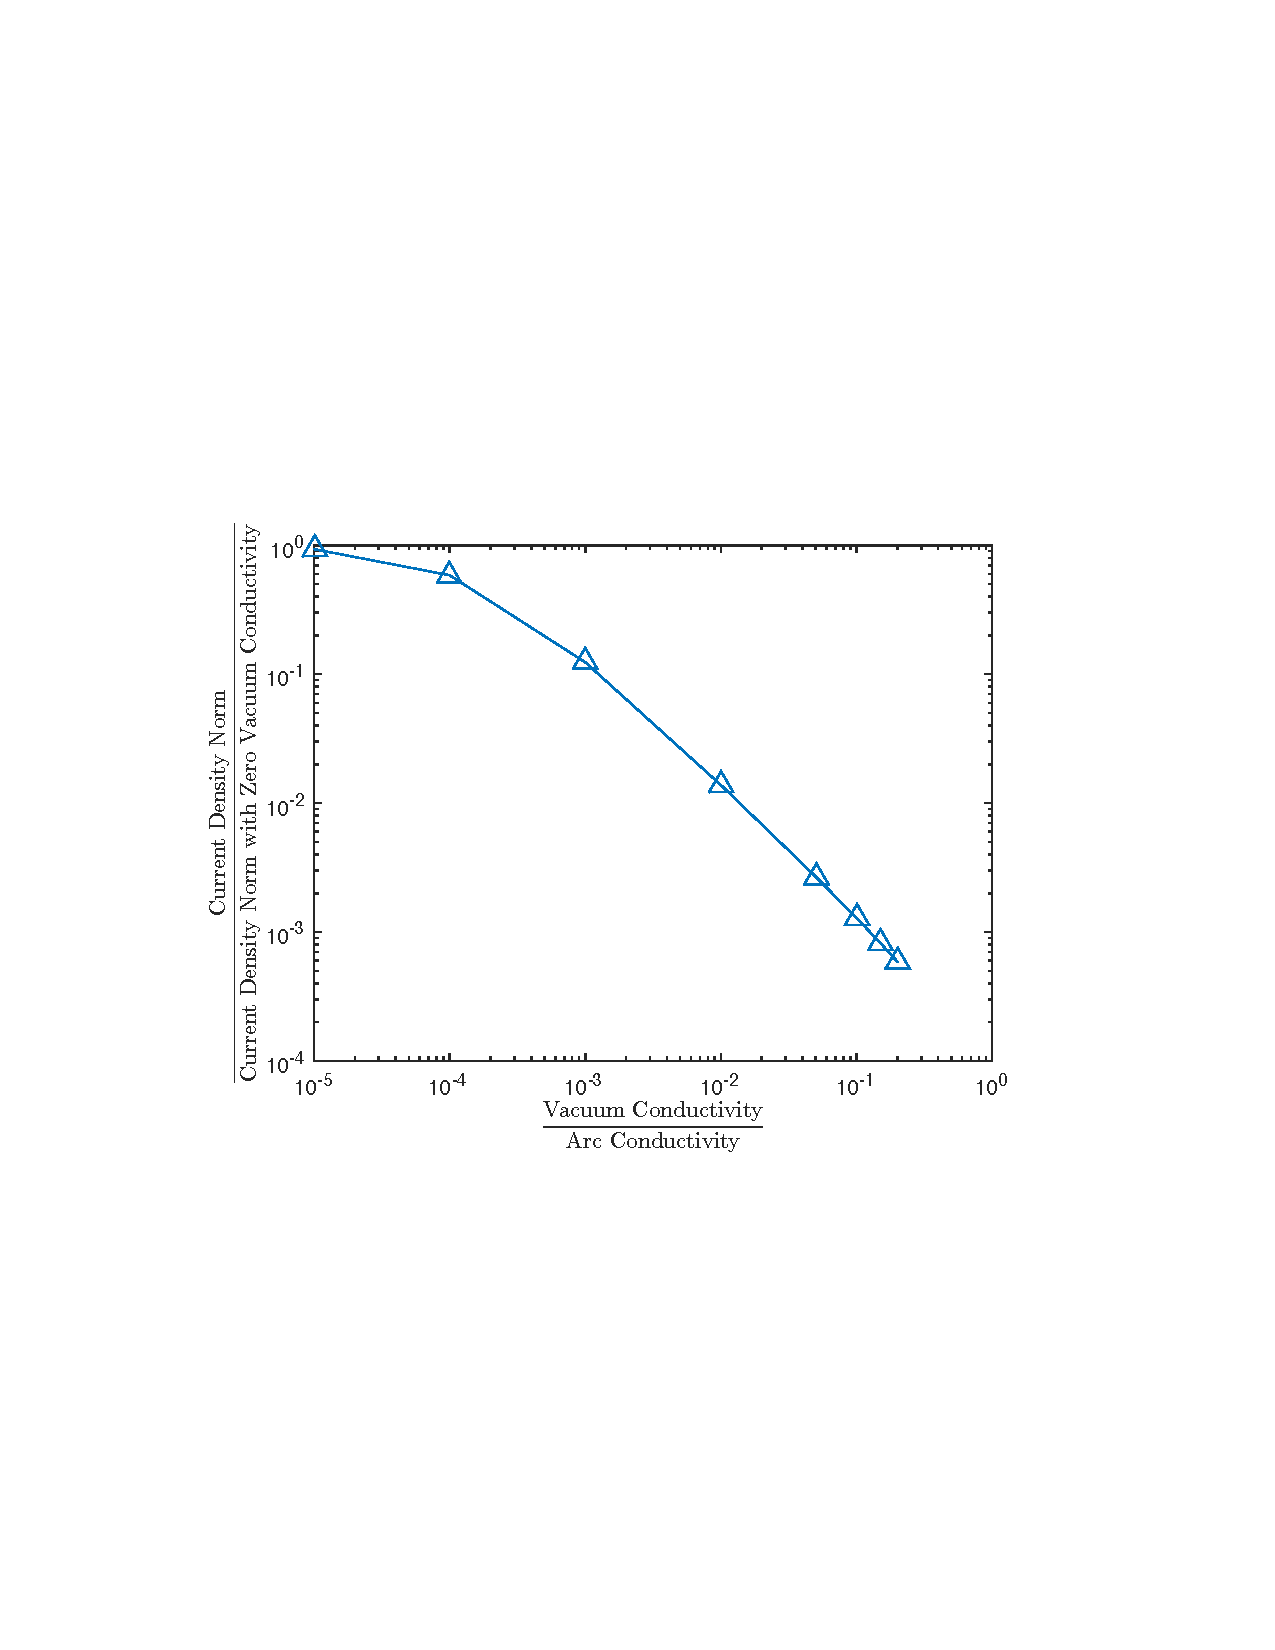
\includegraphics[width=0.6\textwidth]{currentsensitivity.pdf}
%	\caption{Fraction of current density through the arc with varying conductivity of the vacuum chamber material}
%	\label{fig:currentsens}
%\end{figure}

%%%%%%%%%%%%%%%%%%%%%%%%%%%%%%%%%%%%%%%%%%%%%%%%%%%%%%%%%%%%%%%%%%%%%%%%%%%%%%%%%%%%%%%%%%%%%%%%%%%%%%%%%%%%%%%%%%%%%%%%%%%%%%%%%%%

\section{Conclusions}
\label{s:conclusions}

The magnetostatic characteristics of a simplified vacuum arc remelting furnace where studied using the finite element method, in order to determine the effects of various physical phenomena on the resulting magnetic field.
This was done to validate a system for predicting the locations of electrical arcs that form in the electrode-ingot gap in these furnaces.
Arc distribution throughout the remelting process plays a strong role in the material properties of the produced ingot, so real-time tracking of arc locations can provide a priori indications of ingot quality.

First, we reproduced the prior results of Woodside et al.~\cite{Woodside:2013cf} for predicting arc locations; we matched arc location predictions within \SI{3.5}{\percent} of their results.
This minor discrepancy likely resulted from slight differences in model setup, solver version, or selection of input arc locations to calculate the furnace coefficients.
We then studied the effects of changing certain parameters or eliminating previously made assumptions to validate this overall approach for the arc position sensing technology.
Based on our simulations, we drew the following conclusions:
\begin{enumerate}

\item Error in predicted arc locations increases substantially as the sensor moves vertically from the electrode-ingot gap; for distances of \SI{0.508}{\meter} above and below the plane of the gap, the maximum error reached around \SI{40}{\percent} for constant furnace coefficients and \SI{25}{\percent} for adaptive furnace coefficients.
Furthermore, as the sensor moves away from the gap, the magnetic flux density decreases and results in clustering of predicted locations near the center of the domain.

\item Gap height variations do not significantly affect predictions in arc location: varying the gap height from \SI{0.0128}{\meter} to \SI{0.063}{\meter} resulted in the median error changing by \SI{0.55}{\percent} and the maximum error by \SI{1.65}{\percent}.

\item Ingot shrinkage does not affect predictions in arc location; varying the ingot contact zone from the entire length down to \SI{0.032}{\meter} kept the maximum error around \SI{10}{\percent}, and did not change the median error of around \SI{2}{percent}.

\item Averaging the measurements of four evenly spaced sensors around the furnace reduces prediction error distribution by \SI{12.64}{\percent} compared to a single sensor ; there is little to no improvement on location predictions with the implementation of more than four sensors. The total error distribution reduces by \SI{0.85}{\percent} comparing the implementation of four sensors against sixteen. The application of four sensor averaging aids in the suppression of error when taking into account vertical sensor position.

\end{enumerate}

Overall, out of the parameters and assumptions we studied, we conclude that gap height variation and ingot shrinkage will not affect arc location predictions.
However, increasing vertical distance between the sensor and arc will lead to significant errors in location prediction, and should be considered for further development of the arc position sensing technology.

%%%%%%%%%%%%%%%%%%%%%%%%%%%%%%%%%%%%%%%%%%%%%%%%%%%%%%%%%%%%%%%%%%%%%%%%%%%%%%%%%%%%%%%%%%%%%%%%%%%%%%%%%%%%%%%%%%%%%%%%%%%%%%%%%%%





\phantom{}\newpage
\phantom{}\vfill
\begin{center}
\heading
Manuscript 2
\end{center}
\vfill
Miguel F Soler, Kyle E Niemeyer
\vfill\noindent
TBD\\
New York, NY\\
Vol. 1, 100--200
\vfill

\chapter{Manuscript 2}

%%%%%%%%%%%%%%%%%%%%%%%%%%%%%%%%%%%%%%%%%%%%%%%%%%%%%%%%%%%%%%%%%%%%%%%%%%%%%%%%%%%%%%%%%%%%%%%%%%%%%%%%%%%%%%%%%%%%%%%%%%%%%%%%%%%


\section{Abstract}
{\it 

}


%%%%%%%%%%%%%%%%%%%%%%%%%%%%%%%%%%%%%%%%%%%%%%%%%%%%%%%%%%%%%%%%%%%%%%%%%%%%%%%%%%%%%%%%%%%%%%%%%%%%%%%%%%%%%%%%%%%%%%%%%%%%%%%%%%%


\section{Introduction}

\section{Methodology}

In order to solve the problem at hand we need to calculate for fluid flow and heat transfer. 
The finite volume software ANSYS Fluent 17.2 was used to solve for the governing equations. 
The finite volume method was selected because it offers multiple advantages for computational fluid dynamics, mainly how conservation is forced at cell walls and how pressure is coupled using multi-grid solvers.
ANSYS Fluent can be used inside the software ANSYS Workbench, where different solvers can be combined to solve complex multi-physics problems. 
The software is written in C, and offers true dynamic memory allocation, efficient data structures, and flexible solver control. [cite ANSYS guide] 
Fluent uses ANSYS meshing software for mesh generation, which supports the creation of 2D triangular and quadrilateral, as well as 3D tetrahedral, hexahedral, pyramid, wedge, polyhedral, and mixed/hybrid meshes. [cite ANSYS guide] 

\subsection{Governing Equations}
\subsubsection{Continuity and Momentum} 
The flow of the liquid metal portion of the ingot is described by the continuity equation, incompressible form of the Navier-Stokes equations, and the energy equation. The general form of the continuity equations is
\begin{align}
	\frac{\partial \rho}{\partial t} + \nabla \cdot (\rho \mathbf{v}) = S_m
\end{align}

Where $\rho$ is the fluid density, $\mathbf{v}$ is the velocity vector, and $S_m$ is the source term. 
The continuity equation for 2D geometries used here can be written as
\begin{align}
	\frac{\partial \rho}{\partial t} + \frac{\partial}{\partial x}(\rho v_x) + \frac{\partial}{\partial y}(\rho v_y) = S_m
\end{align}

Conservation of momentum in an inertial and non-accelerating reference frame is[cite 25]
\begin{align}
	\frac{\partial}{\partial t}(\rho\mathbf{v}) + \nabla \cdot (\rho \mathbf{v}\mathbf{v}) = -\nabla p + \nabla \cdot(\bar{\bar{\tau}}) + p \mathbf{g} + \mathbf{F}
\end{align}

where $p$ is the static pressure, $\bar{\bar{\tau}}$ is the stress tensor, $p \mathbf{g}$ is the gravitational body force, and $\mathbf{F}$ are the external body forces which for these simulations is zero. 
The stress tensor is defined as
\begin{align}
	\bar{\bar{\tau}} = \mu \Big[(\nabla \mathbf{v} + \nabla \mathbf{v}^{T}) - \frac{2}{3} \nabla \cdot \mathbf{v} I \Big]
\end{align}

where $\mu$ is the molecular viscosity, $I$ is the unit tensor, and the term on the right hand side is the effect of volume dilation. [cite] 
\subsubsection{Turbulence} 
Due to the relatively low viscosity and high density of liquid metals, flow is easily transitioned into the turbulent regime. 
Due to buoyancy driven (in addition to lorentz forces) flow in VAR operation, the melt pool flow exhibits turbulence. [cite Kelkar, Periclous, Gartling]
For this stage of the study we will be neglecting lorentz forces. 
The turbulence model selected for the numerical simulation is the standard $k-\epsilon$ model.
Since being introduced by Launder and Spalding the standard $k-\epsilon$ model has seen widespread use in industry and academia. 
The highlighted benefits are its relatively low memory requirements, robustness, and reasonable accuracy.
The standard $k-\epsilon$ is a two equation model consisting of the turbulence kinetic energy , $k$, and its rate of dissipation, $\epsilon$.

The equation for the turbulence kinetic energy is 
\begin{align}
	\frac{\partial}{\partial t} (\rho k) + \frac{\partial}{\partial x_i} (\rho k u_i) = \frac{\partial}{\partial x_j} \Big[ \Big( \mu + \frac{\mu_t}{\sigma_k}\Big) \frac{\partial k}{\partial x_j} \Big] + G_k + G_b - \rho \epsilon 
\end{align}

where $G_k$ is the rate of production of kinetic energy of turbulence
\begin{align}
	G_k = \mu_t \Big( \frac{\partial u_j}{\partial x_i} + \frac{\partial u_i}{\partial x_j} \Big) \frac{\partial u_j}{\partial x_i}
\end{align}

and $G_b$ is the generation of turbulence due to buoyancy
\begin{align}
	G_b = -g_i \frac{\mu_t}{\rho \sigma_h} \frac{\partial \rho}{\partial x_i}
\end{align}

where $\mu_t$ is the turbulent viscosity and is calculated as follows
\begin{align}
	\mu_t = \rho C_{\mu} \frac{k^2}{\epsilon}
\end{align}	

The equation for the rate of dissipation is
\begin{align}
	\frac{\partial}{\partial t} (\rho \epsilon) + \frac{\partial}{\partial x_i} (\rho \epsilon u_i) = \frac{\partial}{\partial x_j} \Big[ \Big( \mu + \frac{\mu_t}{\sigma_{\epsilon}}\Big) \frac{\partial \epsilon}{\partial x_j} \Big] + C_{1\epsilon}\frac{\epsilon}{k}\Big(G_k + C_{3\epsilon}G_b\Big) - C_{2\epsilon}\rho\frac{\epsilon^2}{k} 
\end{align}

with the standard empirical constants used
\begin{align}
	C_{1\epsilon} = 1.44, \ C_{2\epsilon} = 1.92,\ C_{\mu} = 0.09,\ \sigma_{k} = 1.0,\ \sigma_{\epsilon} = 1.3
\end{align} 

\subsubsection{Solidification}

An enthalpy-porosity technique is used in ANSYS Fluent for the modeling of solidification. 


\subsection{Meshing and Boundary Conditions}

\section{Results}

\section{Conclusion}

\chapter{Conclusion}
Wow, that really was excellent.
\section{Fin}
This is the end, my only friend, the end.


\bibliographystyle{plain}
\bibliography{thesis}

\appendix
\chapter{Redundancy}
This appendix is inoperable.

\end{document}
